\section{Sirona Omnicam Image Acquisition Investigation}

\subsection{Objective and Initial Approach}

The initial objective of this investigation was to obtain image data directly from the \textbf{Sirona Omnicam} for use within the DentaVision project. Access to the scanner's image stream was considered an important prerequisite for eventually integrating the scanner into the reconstruction pipeline and avoiding dependence on externally provided datasets or pre-existing scan data.

The initial approach was based on the assumption that the Omnicam could expose its camera or acquisition interface as a conventional USB device. Therefore, the first step was to investigate how the scanner was connected to the computer and whether its USB interface could provide a direct path to the acquired images. Both the \code{Windows Device Manager} and \code{USBTreeView} were used for this purpose. The connected devices and USB interfaces were inspected in an attempt to identify an entry corresponding to the Sirona Omnicam, or a device with a name or hardware information that could be associated with the scanner. USBTreeView was additionally used to inspect the available USB device information, interfaces, and endpoints in greater detail. This initial investigation did not provide a straightforward way to access the scanner's image data. In particular, identifying the device at the USB level did not imply that the image stream was exposed through a standard camera interface that could be accessed independently of the manufacturer's software. This led to a change in the investigation strategy.

Instead of treating the Omnicam as a conventional USB camera, the investigation was subsequently expanded to the \code{hardware, camera interfaces, drivers, acquisition SDK, and CEREC software stack}. The purpose was to determine how the scanner was actually exposed to the operating system and how the CEREC software interacted with the underlying hardware. This ultimately led to the investigation of the Matrix Vision camera components and, later, to reverse engineering of the software and DLLs used by \textbf{CEREC SW 5.1}.

\subsection{Camera and Acquisition Interface Investigation}

After the initial USB-level investigation, the focus shifted towards identifying the camera hardware used by the Omnicam and determining whether it could be accessed independently of the CEREC software. The investigation revealed that the scanner contained an industrial camera from MATRIX VISION, identified as a SiCamCCT camera belonging to the mvBlueCOUGAR family. The device was identified with serial number 27323555 and exposed a GenICam interface. The camera used an ICX424 sensor and communicated through GigE Vision.

The identification of the camera was significant because it provided a potential acquisition interface that could be investigated independently of the higher-level CEREC software. The Matrix Vision ecosystem includes tools and libraries for configuring and acquiring images from compatible devices. Therefore, the investigation focused on the mvIMPACT Acquire SDK and the associated wxPropView utility.

\subsubsection{Camera Detection and SDK Investigation}

The mvIMPACT Acquire SDK was used to investigate whether the camera could be detected and accessed directly. The device could be identified through the Matrix Vision acquisition software, confirming that the underlying camera hardware was accessible at this level. Several Matrix Vision components were also identified as being associated with the device, including libraries such as \code{mvDeviceManager.dll}, \code{mvBlueCOUGAR.dll} and \code{mvPropHandling.dll}. The wxPropView application was additionally used to inspect and configure the available camera properties. This provided access to acquisition-related parameters and helped determine whether the camera could be operated outside the normal CEREC acquisition workflow. The investigation also identified several image formats supported by the camera interface, including:

\begin{itemize}
    \item \code{RGB8Packed}
    \item \code{RGB20p12}
    \item \code{BGR8Packed}
    \item \code{BGR10V2Packed}
\end{itemize}

The availability of these formats indicated that the camera interface itself was capable of providing image data in standard color representations. However, this did not necessarily mean that the Omnicam used these formats during its normal scanning operation.

\subsubsection{Acquisition Attempts}

Despite successfully detecting the camera and accessing its configuration through the Matrix Vision tools, obtaining a usable image through direct acquisition initially proved unsuccessful. One of the main observed results was a black image being returned during acquisition attempts. This indicated that device detection and communication with the camera did not necessarily imply that the complete acquisition process used by the Omnicam had been correctly reproduced.

Acquisition parameters, particularly exposure-related settings, were investigated and adjusted in an attempt to determine whether the black image was caused by an incorrect configuration. A newer version of the mvIMPACT Acquire SDK was also installed and tested. After experimenting with different exposure settings and other available acquisition parameters, it was eventually possible to obtain an image in grayscale. However, this result did not provide a reliable acquisition path suitable for integration into an automated scanning pipeline. In addition, the mvIMPACT Acquire SDK did not provide a mechanism to control the scanner's projector, which was an important limitation because image acquisition alone would not be sufficient to reproduce the structured-light scanning process used by the Omnicam.

\subsubsection{Result and Limitations}

The investigation established that the Omnicam contained an identifiable Matrix Vision industrial camera that could be detected and accessed at the SDK level. The GenICam, GigE Vision, and mvIMPACT Acquire interfaces therefore provided a real hardware-level access point for further investigation. However, direct access to the camera through these interfaces was not sufficient to reproduce the scanner's normal image acquisition. Although a grayscale image could eventually be obtained, the acquisition process could not be demonstrated to provide the complete set of functionality required for automated scanning. In particular, the inability to control the scanner's projector through the available SDK represented a significant limitation. At this stage, the investigation therefore shifted from attempting to operate the camera solely through the Matrix Vision acquisition interface towards understanding how the CEREC software and its associated components controlled and interacted with the scanner.

\subsubsection{Investigation Method: Software Interaction and Reverse Engineering}

After the direct acquisition approach through the Matrix Vision interfaces failed to provide a complete and reliable way of obtaining the images required for the project, the investigation shifted towards understanding how the original CEREC software interacted with the scanner.

The main objective of this phase was to identify the software components responsible for communicating with and controlling the Omnicam and to determine whether the scanner's acquisition process could be reproduced or controlled outside the original CEREC environment. Particular attention was given to the possibility that the CEREC software performed additional operations that were not exposed through the standard Matrix Vision acquisition SDK.

The investigation began by examining the components used by CEREC SW 5.1 during scanner operation. Process Monitor was used to observe the activity of the software while interacting with the scanner. This provided information about the processes, dynamic-link libraries, files, and other system resources involved during the acquisition workflow. The collected information was used to identify potentially relevant components for further analysis. The identified binaries were subsequently investigated using Ghidra. The purpose of the reverse-engineering process was not to fully reconstruct the entire CEREC software, but to identify relevant functions, classes, data structures, and relationships that could provide information about the scanner's acquisition pipeline. Particular attention was given to the following DLLs:

\begin{itemize}
    \item \code{acquire.dll}
    \item \code{CAI2_CameraCCT.dll}
    \item \code{SiAcquireCtrl.dll}
    \item \code{mvPropHandling.dll}
    \item \code{MHT_ScannerLib.dll}
\end{itemize}

The analysis focused on finding evidence of functionality related to several stages of the scanning process. These included scanner initialization, starting and stopping the scanning process, image acquisition, and the transfer or processing of acquired data. In addition, the investigation specifically looked for code that could provide information about the structured-light system, particularly functions or components related to projector control, pattern generation or sequencing, and synchronization between the projected patterns and camera acquisition.

The latter aspects were particularly relevant because obtaining camera frames alone would not necessarily reproduce the Omnicam's scanning process. If the scanner relies on structured-light patterns, the acquired images would need to be synchronized with the corresponding projected patterns in order to reproduce the same type of measurement outside the original software. The reverse-engineering results were therefore used to construct a partial model of the scanner's software and data flow. Because this analysis was based primarily on decompiled binaries and indirect relationships between functions and components, the resulting architecture was treated as a set of working hypotheses rather than as a definitive description of the scanner's internal implementation. 

The analysis was also subject to significant practical limitations. The CEREC software consisted of numerous interconnected binaries and libraries, and not all components could be interpreted reliably or easily from their decompiled representation. Indirect calls, complex dependencies, compiler-generated structures, and the amount of available code made it difficult to follow the complete execution path. Consequently, the investigation was able to identify several relevant components and data flows, but it was not possible to reconstruct the complete scanner acquisition and reconstruction pipeline with certainty.

\subsection{Reverse Engineering Findings and Working Hypotheses}

The reverse-engineering analysis provided evidence of several components and data paths involved in the Omnicam's scanning process. However, the following reconstruction should not be understood as a definitive description of the scanner's internal architecture. It was derived primarily from decompiled binaries, identified class and function relationships, and the interpretation of data structures and buffers. Consequently, some elements are directly supported by the analyzed code, while others represent working hypotheses based on the observed relationships.

\subsubsection{Identified Components}

One of the main components identified during the analysis was \code{ScannerProxy}, which appears to provide a high-level abstraction of the scanner hardware. The analyzed code contains functions such as \code{ScannerProxy::StartScanning(bool enable)}, \longcode{ScannerProxy::CreateUsbScanData2D(...)}, and \longcode{ScannerProxy::CreateUsbScanData25D(...)}. The class also appears to provide access to a \code{MainFpgaProxy} object through a virtual function call. Based on the analyzed relationships, \code{ScannerProxy} was interpreted as a component connecting several parts of the acquisition process, including camera acquisition, FPGA-related processing, and the creation of scan-data objects. \code{MainFpgaProxy} appears to represent an interface to the scanner's internal FPGA. Among the identified functions are \longcode{IsInterpolatedPeaksUsbData()}, \longcode{motor\_hard\_stop\_front\_in\_micrometers()}, and \longcode{motor\_hard\_stop\_back\_in\_micrometers()}. The presence of these functions suggests that the FPGA interface is associated not only with data processing but also with aspects of the scanner's mechanical control.

The analysis also identified a hierarchy of scan-data objects. \code{ScanData} appears to act as a high-level container holding references to two different types of data, which were interpreted as \code{ScanData2D} and \code{ScanData25D}. The constructors observed in the decompiled code copy two independent \code{shared_ptr} objects, which is consistent with such a structure, although the complete original class definition could not be recovered. \code{ScanData2D} appears to represent the two-dimensional camera data. The function \code{ScanDataHelper::GetRawTwoDScanData()} was identified together with parameters corresponding to image width, height, and a raw data buffer. The analysis also identified. \longcode{TwoDCameraProcess::DebayerBayeredImage()}, providing evidence for a Bayer image processing stage. \code{ScanData25D}, in contrast, appears to represent processed data associated with the scanner's three-dimensional acquisition. The analyzed code distinguishes between raw and interpolated peak data. Depending on the selected mode, the data appears to be encapsulated in either \code{UsbScanData25D} or \code{UsbScanData25DInterpolatedPeaks}. Several constructors associated with these objects were also identified:

\begin{itemize}
    \item \code{FUN_180177750} $\rightarrow$ \code{UsbScanData25D}
    \item \code{FUN_180177850} $\rightarrow$ \longcode{UsbScanData25DInterpolatedPeaks}
    \item \code{FUN_180177960} $\rightarrow$ \code{UsbScanData2D}
    \item \code{FUN_180183310} $\rightarrow$ \code{UsbScanData2D}
\end{itemize}

These functions were interpreted as object constructors rather than as functions performing the actual three-dimensional reconstruction.

\subsubsection{Identified Data Paths}

The analysis provided stronger evidence for the two-dimensional camera-data path than for the complete three-dimensional reconstruction pipeline. The identified camera configuration and the observed \longcode{TwoDCameraProcess::DebayerBayeredImage()} call suggest that the scanner can acquire image data in a Bayer mosaic representation before converting it to RGB through software processing. The corresponding data path can therefore be represented as:

\[
\text{Camera}
\rightarrow
\text{RAW Bayer}
\rightarrow
\text{Debayer}
\rightarrow
\text{RGB}
\]

This interpretation is supported by the identification of the Bayer acquisition mode and the explicit debayering function in the analyzed code. 

The creation of \code{ScanData2D} also provided evidence of a raw byte buffer being passed into the scanner's data structures. In particular, \longcode{ScannerProxyQcc61::CreateUsbScanData2D(...)} accepts a \code{shared_ptr<vector<unsigned char>>} together with image dimensions. During the construction process, an ROI object was also observed, suggesting that the useful image region may be defined at this stage. The exact role and contents of all associated metadata, however, could not be established with certainty.

A separate data path appears to originate from the FPGA. The analyzed code distinguishes between raw peaks and interpolated peaks, controlled by the result of \longcode{MainFpgaProxy::IsInterpolatedPeaksUsbData()}. The corresponding conceptual flow was interpreted as:

\[
\resizebox{\columnwidth}{!}{$
\text{FPGA}
\rightarrow
\text{Raw or Interpolated Peak Data}
\rightarrow
\text{ScanData25D}
$}
\]

The observed object sizes were approximately 12,776 bytes (\code{0x31E8}) for the normal representation and 10,760 bytes (\code{0x2A08}) for the interpolated representation. These values provide evidence that different internal data representations are used, although their complete binary structure was not determined.

Overall, the analyzed code suggests that the scanner handles at least two related data streams: a two-dimensional camera stream and a second stream containing peak or height-related information. These streams are subsequently represented through the \code{ScanData2D} and \code{ScanData25D} structures.

\subsubsection{Partial Reconstruction of the Acquisition Flow}

Based on the identified functions and relationships, a partial reconstruction of the acquisition flow was developed. When the user initiates a scan, \code{ScannerProxy::StartScanning(bool enable)} appears to initiate or enable the scanning process. During this process, the \code{ScannerProxy} is associated with both camera-related functionality and the \code{MainFpgaProxy}. The analyzed relationships suggest the following conceptual flow:

\[
\resizebox{\columnwidth}{!}{$
\text{Scan Initiation}
\rightarrow
\text{ScannerProxy::StartScanning()}
\rightarrow
\begin{cases}
\text{Camera Acquisition}\\
\text{FPGA-related Processing}
\end{cases}
$}
\]

The camera-related path appears to produce RAW Bayer data that is subsequently processed through software debayering and represented as \code{ScanData2D}. In parallel, the FPGA-related path appears to produce peak or height-related data that is represented as \code{ScanData25D}. This can be summarized as:

\[
\resizebox{\columnwidth}{!}{$
\begin{array}{ccc}
& \text{ScannerProxy} & \\
& \swarrow \qquad \searrow & \\\\
\text{Camera} && \text{Main FPGA} \\
\downarrow && \downarrow \\
\text{RAW Bayer} && \text{Peak/Height Data} \\
\downarrow && \downarrow \\
\text{ScanData2D} && \text{ScanData25D} \\
\downarrow && \downarrow \\
\text{Debayer / RGB} && \text{Processed 2.5D Data}
\end{array}
$}
\]

This represents a working model rather than a fully verified implementation. In particular, the analysis did not establish that \code{StartScanning()} itself directly controls every stage of the acquisition process. Instead, it appears to initiate a larger sequence in which other modules perform the camera, FPGA, and potentially optical operations. The presence of the message ``Generating faked volume data!'' during the analysis of \code{StartScanning()} also suggests that the software contains an internal simulation or testing mode capable of generating artificial volume data. This provides additional evidence that the scanner software contains different internal acquisition and processing paths, although the exact purpose and activation conditions of this mode could not be fully established.

\subsubsection{Inferred Working Model of the Acquisition and Data Flow}

Based on the available evidence, the following model represents the most plausible interpretation of the scanner's acquisition architecture at the time of the investigation:

\begin{figure}[H]
    \centering
    \resizebox{\columnwidth}{!}{%
    \begin{tikzpicture}[
        node distance=8mm and 18mm,
        box/.style={
            draw,
            rounded corners,
            align=center,
            minimum width=30mm,
            minimum height=9mm
        },
        arrow/.style={
            -{Stealth},
            thick
        }
    ]

        % Top
        \node[box] (projector) {Projector\\(inferred)};

        \node[box, below=of projector] (patterns)
            {Structured-Light Patterns};

        \node[box, below=of patterns] (object)
            {Scanned Object};

        % Camera and FPGA branches
        \node[box, below left=12mm and 18mm of object] (camera)
            {SiCamCCT Camera\\RAW Bayer};

        \node[box, below right=12mm and 18mm of object] (fpga)
            {Main FPGA\\Peak / Height Data};

        \node[box, below=of camera] (scan2d)
            {ScanData2D};

        \node[box, below=of fpga] (scan25d)
            {ScanData25D};

        \node[box, below=of scan2d] (debayer)
            {Debayer / RGB};

        \node[box, below=of scan25d] (processed)
            {Processed 2.5D Data};

        % Merge
        \node[box, below=16mm of object] (scandata)
            {ScanData};

        \node[box, below=of scandata] (processing)
            {Subsequent 3D Processing};

        \node[box, below=of processing] (output)
            {Point Cloud / Mesh};

        % Arrows
        \draw[arrow] (projector) -- (patterns);
        \draw[arrow] (patterns) -- (object);

        \draw[arrow] (object) -- (camera);
        \draw[arrow] (object) -- (fpga);

        \draw[arrow] (camera) -- (scan2d);
        \draw[arrow] (fpga) -- (scan25d);

        \draw[arrow] (scan2d) -- (debayer);
        \draw[arrow] (scan25d) -- (processed);

        % Merge into ScanData
        \draw[arrow] (debayer) -- (scandata);
        \draw[arrow] (processed) -- (scandata);

        \draw[arrow] (scandata) -- (processing);
        \draw[arrow] (processing) -- (output);

    \end{tikzpicture}%
    }
    \caption{Inferred data flow of the Omnicam scanning pipeline.}
    \label{fig:omnicam-data-flow}
\end{figure}

The camera, FPGA, \code{ScanData2D}, and \code{ScanData25D} relationships shown in this model are supported to varying degrees by the analyzed code. The projector, structured-light pattern generation, synchronization, and final three-dimensional processing are included as inferred components rather than confirmed findings.

\subsubsection{Unresolved Components and Limitations}

Despite identifying several important components, significant parts of the acquisition pipeline remained unresolved. The most important unresolved component was the projector control. The analysis did not identify explicit functions or modules clearly associated with terms such as \code{Projector}, \code{Pattern}, \code{GrayCode}, \code{PhaseShift}, \code{DLP}, \code{Sequence}, \code{Projection}, \code{LED}, or \code{Laser}. Consequently, no direct evidence was found showing where the structured-light patterns were generated or how the projector was controlled. Similarly, the synchronization mechanism between the projector and camera could not be identified. A complete automated acquisition process would likely require coordination between the projected pattern and the corresponding camera exposure, but the specific mechanism responsible for this synchronization remained unknown. The exact format of the internal data buffers was another unresolved aspect. Although several buffers were identified as \code{vector<unsigned char>} objects and their approximate sizes could be determined, their internal fields could not be fully reconstructed. Elements such as headers, frame identifiers, timestamps, peak values, calibration information, or coordinates could therefore not be confirmed. The final processing stages were also not fully identified. Although the presence of \code{ScanData25D} suggests that data related to three-dimensional acquisition is generated before later processing, the exact component responsible for transforming this information into a point cloud, mesh, or final three-dimensional model was not established.

Finally, the reverse-engineering process itself imposed substantial limitations. The CEREC software consisted of numerous interconnected DLLs, and several binaries were difficult to interpret reliably using decompilation. Indirect calls, compiler-generated structures, dependencies between modules, and the complexity of the assembly code made it difficult to trace complete execution paths. As a result, the analysis was sufficient to identify several relevant components and construct a plausible working model, but not to verify the complete internal architecture of the Omnicam with certainty or to identify a self-contained function that could be invoked from custom software to initiate and reproduce the complete scanning process.


\subsection{UDP Communication and Data Capture Investigation}

\subsubsection{Initial UDP Communication and API Prototype}

During the investigation of the scanner control commands, a small prototype API was developed in parallel to explore how a programmable scanner interface could be structured if a suitable command for initiating the scan could be identified. At this stage, it was still assumed that such a command might be available and that it could potentially be integrated into a custom acquisition interface. The intended concept was to provide an interface capable of connecting to the scanner, initiating a scan through a command identified during the reverse-engineering process, receiving the resulting data, and subsequently forwarding it to the DentaVision processing pipeline. The objective was therefore not to provide a complete scanner implementation, but to investigate the software structure that could be used for such an interface. The prototype introduced an abstract hardware interface with operations for connecting to the scanner, projecting a pattern, capturing an image, and disconnecting from the device. A mock implementation was used to simulate these operations and to verify the intended control flow. A higher-level \code{Scanner} class could then execute a sequence consisting of connecting to the hardware, projecting several patterns, capturing the corresponding images, and disconnecting. This prototype was developed as a preliminary representation of the intended scanner-control architecture rather than as a functional interface to the physical Omnicam. Once the investigation progressed and no suitable command for independently initiating the scanning process could be identified, the prototype was no longer pursued as a means of controlling the physical scanner.

\subsubsection{Investigation and Reproduction of GVCP Commands}

As the reverse-engineering analysis had not identified a directly usable function for starting the scan from custom software, the network communication between the scanner and the CEREC software was investigated. The motivation for this approach came from observing the network activity of the system during a scan. In the Windows Task Manager, Ethernet usage increased noticeably when a scan was initiated in the CEREC software, suggesting that a significant amount of data could be exchanged through the network interface. This raised the possibility that the scanner might communicate with the CEREC software over the network, leading to the use of Wireshark to capture and investigate the corresponding traffic. Wireshark was used to observe the UDP traffic generated during scanner operation. Particular attention was given to communications occurring before and around the beginning of a scan, with the objective of identifying commands that could potentially be reproduced independently of the original software.

Based on this investigation, a C++ implementation of a UDP communication layer was developed. The \code{UDPClient} class provided basic UDP packet transmission and reception, while \code{GvcpClient} implemented read and write operations for registers using the observed GVCP command structure. A \code{GvcpSequence} class was additionally implemented to execute a series of register operations in a defined order.
Several register addresses were investigated and sequences containing read and write operations were tested. The scanner responded to some of the transmitted commands, demonstrating that communication with the device could be established through the implemented UDP interface. However, reproducing the complete sequence required to initiate the scanning process was not achieved. Consequently, although the experiment demonstrated that the scanner could respond to custom UDP/GVCP communication, it did not provide a reliable method for starting an acquisition independently from the CEREC software.

\subsubsection{Direct Capture of Scanner Data}

After the attempt to initiate the scanning process through reproduced commands was unsuccessful, a different approach was investigated. Instead of attempting to control the scanner directly, the CEREC software was used to initiate the scan manually while the custom program listened for the data transmitted by the scanner. A UDP receiver was implemented in C++ specifically for this purpose. The \code{GvspReceiver} class opened a UDP socket on the investigated GVSP port and waited for incoming datagrams. The received packets were inspected to extract information interpreted as block identifiers, packet identifiers, and packet types. The receiver attempted to distinguish between leader, data, and trailer packets and to group packets belonging to the same block. Data packets were then processed by removing the interpreted packet header and appending the remaining bytes to an output buffer. The accumulated data were subsequently written to a binary file named \code{frame.raw}. In addition, a separate \code{GvspAnalyzer} component was implemented to inspect previously captured data. It divided the captured stream into fixed-size packets and reported the interpreted block and packet identifiers, allowing the structure and continuity of the received data to be investigated. This implementation therefore demonstrated that data transmitted by the scanner could be captured independently of the CEREC application's normal display path and stored for further analysis.

\subsubsection{Observed Behaviour During Data Capture}

An important observation was made while performing the direct data-capture experiment. When the custom receiver was connected to the investigated communication port and started receiving the scanner's transmitted data, the live image that normally appeared in the CEREC software stopped being displayed. This behaviour was considered potentially significant because it suggested that the captured traffic could be related to the data stream used by the scanner during acquisition. However, the observation alone was not sufficient to establish that the received packets represented the camera images directly.

In particular, the internal architecture analysis had already indicated that the scanner may exchange multiple types of data associated with the acquisition and 3D reconstruction process. Therefore, the captured stream could potentially contain image data, processed 3D-related data, metadata, or a combination of different data types. The possibility of additional encoding or an undocumented internal data format also could not be excluded. Consequently, the disappearance of the live image was treated as an indication that the captured traffic was relevant to the scanner's acquisition process, rather than as definitive evidence that the received bytes constituted directly usable image frames.

\subsubsection{Data Interpretation and Limitations}

Although the C++ receiver successfully captured and stored data transmitted by the scanner, the complete structure and meaning of the received stream could not be established. The captured binary data could not be reliably reconstructed into usable image frames. The investigation therefore did not establish whether the received data consisted exclusively of camera images, contained a combination of image and 3D-related information, or used an additional encoding or proprietary representation. The packet-level analysis provided information about the apparent structure of the communication, but it was insufficient to reconstruct the complete payload semantics.
As a result, the \code{frame.raw} output should be understood as a capture of received binary data rather than as a successfully reconstructed image.

Combined with the lack of a reliable method for initiating the scan programmatically, the limited available documentation, and the difficulty of determining the internal data representation, this approach was ultimately considered impractical for obtaining image data from the Omnicam for the DentaVision pipeline. The scanner was therefore not used as the image source for the subsequent development. Instead, image acquisition was moved to the project's virtual/simulated pipeline, where the required camera input could be provided while allowing the remaining DentaVision processing and reconstruction pipeline to be developed independently of the limitations encountered with the physical scanner.

\subsection{Conclusion and Future Considerations}

The investigation successfully identified the main camera hardware and acquisition interfaces, provided access to relevant device information, examined the available SDKs, identified several relevant software components, and allowed parts of the scanner's acquisition and data flow to be inferred through reverse engineering. It was also possible to establish UDP communication with the scanner and capture data transmitted during an acquisition. However, no reliable method was found to obtain directly usable images for the DentaVision pipeline, fully control the scanner, identify the synchronization mechanism of the structured-light system, or completely interpret the captured data.

As a result, the investigation of direct image acquisition from the Omnicam was concluded, and the scanner was not used as the image source for the subsequent development of DentaVision. Nevertheless, the work provided a partial understanding of the scanner's internal architecture and identified several relevant acquisition and processing paths. For future investigations, the use of a programmable scanner with documented access to its acquisition process would be preferable.


% 3d reconstruction
\section{3D Reconstruction}

\subsection{Theoretical Background}

Three-dimensional reconstruction from images can be approached through different computer vision paradigms. The methods investigated in this project range from feature-based reconstruction and Structure-from-Motion (SfM) to classical stereo matching and learning-based stereo estimation. Although these approaches differ in their assumptions and internal processing, they all rely on establishing relationships between different observations of the same scene in order to infer three-dimensional information.

The following sections introduce the main concepts required to understand the reconstruction methods implemented and evaluated in this work. The discussion begins with feature-based correspondence using the Scale-Invariant Feature Transform (SIFT), followed by Structure-from-Motion, classical stereo vision and disparity estimation, and finally learning-based stereo matching using IGEV-Stereo.

\subsubsection{Feature-Based Reconstruction and SIFT}

Feature-based reconstruction relies on identifying distinctive visual structures in one or more images and establishing correspondences between observations of the same physical points. These correspondences provide the basis for estimating geometric relationships between images and, ultimately, recovering three-dimensional information about the observed scene.

A typical feature-based pipeline consists of two main stages: feature detection and feature description. First, visually distinctive locations, commonly referred to as \textit{keypoints}, are identified within each image. A descriptor is then computed for the local image region surrounding each keypoint. The descriptors can subsequently be compared between images to determine which keypoints are likely to represent the same physical location. One of the most widely used feature extraction methods is the Scale-Invariant Feature Transform (SIFT), introduced by Lowe \cite{lowe_distinctive_2004}. SIFT detects distinctive image features across different scales and computes a descriptor that characterizes the local appearance around each detected keypoint. An important property of the method is its invariance to image scale and rotation, while also providing robustness to moderate changes in viewpoint, illumination, noise and affine distortion \cite{lowe_distinctive_2004}.

After features have been extracted from multiple images, their descriptors can be compared to establish candidate correspondences. These correspondences are subsequently filtered using geometric constraints in order to remove incorrect matches. The resulting set of reliable correspondences can then be used by higher-level reconstruction algorithms to estimate camera motion or recover the three-dimensional position of observed points. In the context of three-dimensional reconstruction, SIFT therefore does not directly generate a three-dimensional model. Instead, it provides the feature correspondences required by subsequent geometric operations such as pose estimation and triangulation. This distinction is particularly relevant to the reconstruction approaches investigated in this project, where SIFT was used as the basis for both pairwise reconstruction and Structure-from-Motion pipelines.

An inherent limitation of feature-based reconstruction is its dependence on the availability of sufficiently distinctive visual features. Regions with little texture, homogeneous appearance or repetitive structures may provide fewer reliable keypoints and correspondences. As a result, the performance of feature-based approaches can vary considerably depending on the visual characteristics of the observed scene. This limitation motivated the subsequent evaluation of alternative reconstruction approaches based on stereo disparity estimation.

\subsubsection{Structure-from-Motion}

Structure-from-Motion is a computer vision approach that estimates the three-dimensional structure of a scene together with the relative positions and orientations of the cameras from multiple images. Starting from correspondences between image features, SfM jointly recovers the geometry of the observed scene and the motion or pose of the cameras that captured it \cite{szeliski_computer_2022,schonberger_structure--motion_2016}.
A simplified SfM pipeline can be described as follows:

\begin{center}
\resizebox{\columnwidth}{!}{%
\begin{tikzpicture}[
    box/.style={
        rectangle,
        draw,
        rounded corners,
        align=center,
        minimum width=3.0cm,
        minimum height=0.9cm
    },
    arrow/.style={
        ->,
        >=stealth
    }
]

\node[box] (images) {Images};
\node[box, right=0.8cm of images] (detection) {Feature Detection};
\node[box, right=0.8cm of detection] (matching) {Feature Matching};
\node[box, right=0.8cm of matching] (verification) {Geometric Verification};

\node[box, below=1.2cm of verification] (pose) {Camera Pose Estimation};
\node[box, left=0.8cm of pose] (triangulation) {Triangulation};
\node[box, left=0.8cm of triangulation] (reconstruction) {3D Reconstruction};

\draw[arrow] (images) -- (detection);
\draw[arrow] (detection) -- (matching);
\draw[arrow] (matching) -- (verification);

\draw[arrow] (verification) -- (pose);
\draw[arrow] (pose) -- (triangulation);
\draw[arrow] (triangulation) -- (reconstruction);

\end{tikzpicture}%
}
\end{center}

The process begins by detecting and matching features between images. The resulting correspondences are used to estimate the geometric relationship between different camera views. In the case of calibrated cameras, this relationship can be represented through the essential matrix, which encodes the relative rotation and translation between two camera views. Once the relative camera poses have been estimated, corresponding image observations can be triangulated to estimate the three-dimensional position of the observed points. The reconstructed three-dimensional points are commonly referred to as \textit{landmarks}. In multi-view reconstruction, the same landmark may be observed in several images. Maintaining the association between these individual observations and their corresponding three-dimensional points requires the management of \textit{tracks}, which represent groups of feature observations that are assumed to correspond to the same physical point. As additional images are incorporated into the reconstruction, the estimated camera poses and three-dimensional landmarks are refined through bundle adjustment. Bundle adjustment jointly optimizes the reconstruction parameters in order to minimize the reprojection error between the observed image features and the projections of the estimated three-dimensional points \cite{szeliski_computer_2022}.

Although the individual operations involved in SfM can be implemented using general-purpose computer vision libraries, constructing a complete and robust SfM pipeline requires managing feature correspondences, tracks, camera poses, landmarks and iterative optimization. Modern SfM systems therefore integrate these operations into specialized reconstruction pipelines. For example, Schönberger and Frahm describe an incremental Structure-from-Motion pipeline designed to improve robustness, accuracy, completeness and scalability when reconstructing scenes from unordered image collections \cite{schonberger_structure--motion_2016}. This complexity was directly relevant to the development of the reconstruction pipeline in this project. An initial manual implementation demonstrated that performing individual operations such as feature matching, pose estimation and triangulation was not sufficient to construct a complete multi-view reconstruction system without additionally managing the relationships and consistency between all observations. Consequently, established SfM and multi-view reconstruction tools were later investigated as an alternative to implementing the complete pipeline manually.

\subsubsection{Stereo Vision and Disparity}

Stereo vision estimates three-dimensional information by observing the same scene from two different viewpoints. In a stereo camera configuration, two cameras observe the scene from slightly different positions. Consequently, the projection of the same physical point appears at different image locations in the left and right images. After the stereo images have been rectified, corresponding points are typically located along the same horizontal image coordinate. This simplifies the correspondence problem by reducing the search for matching points primarily to the horizontal direction. The horizontal displacement between corresponding points is referred to as \textit{disparity}.
For a rectified stereo pair, disparity can be expressed as

\begin{equation}
d = x_L - x_R
\label{eq:disparity}
\end{equation}

where \(x_L\) and \(x_R\) represent the horizontal coordinates of corresponding points in the left and right images, respectively. The estimated disparity is inversely related to the depth of the observed point. For an ideal stereo configuration, depth can be calculated as

\begin{equation}
Z = \frac{fB}{d}
\label{eq:depth_from_disparity}
\end{equation}

where \(Z\) represents the depth, \(f\) is the focal length, \(B\) is the baseline between the two camera centers, and \(d\) is the disparity. Therefore, points with a larger disparity are generally located closer to the cameras, whereas points with a smaller disparity are located farther away \cite{opencv_depth_map_stereo, opencv_camera_calibration}.

The main challenge in stereo reconstruction is the correspondence problem: determining which pixel or image region in the left image corresponds to the same physical point in the right image. Stereo matching algorithms estimate these correspondences and generate a \textit{disparity map}, in which each valid pixel is associated with an estimated horizontal displacement. Classical stereo matching methods generally combine a matching cost with spatial regularization. The matching cost evaluates the similarity between candidate image regions, while the regularization process encourages geometrically consistent disparity estimates across neighboring pixels. One influential approach is Semi-Global Matching (SGM), proposed by Hirschmüller \cite{hirschmuller_stereo_2008}. SGM approximates global energy optimization by aggregating matching costs along multiple paths through the image while incorporating smoothness constraints. This allows the method to balance local image similarity with spatial consistency without performing a computationally expensive global optimization.

The Stereo Semi-Global Block Matching implementation provided by OpenCV, referred to as StereoSGBM, follows this general class of stereo matching approaches and was used in this project to generate disparity maps from rectified stereo image pairs. The resulting disparity estimates were subsequently used to reconstruct depth and three-dimensional point clouds. Unlike Structure-from-Motion, which estimates camera motion and scene structure from multiple observations, stereo reconstruction can directly estimate depth from the disparity between two views when the relevant camera parameters and stereo geometry are known. This makes stereo matching particularly suitable for evaluating the reconstruction of individual image pairs.

\subsubsection{Learning-Based Stereo Matching and IGEV}

Classical stereo matching methods rely on explicitly designed similarity measures and optimization strategies to establish correspondences between stereo images. Their performance can be affected by ambiguous correspondences, low-texture regions, repetitive patterns and other image characteristics that make it difficult to identify corresponding pixels reliably. Learning-based stereo matching approaches address the correspondence problem by using neural networks trained on stereo data. Instead of relying exclusively on manually designed image features or matching costs, these methods learn feature representations and correspondence relationships from training data. During inference, a trained model receives a stereo image pair and estimates a disparity map representing the relative displacement between corresponding pixels.

One such method is IGEV-Stereo, proposed by Xu et al. \cite{xu_iterative_2023}. IGEV-Stereo introduces the Iterative Geometry Encoding Volume, a representation designed to combine geometric and contextual information with local matching information. The resulting representation is used iteratively to refine the estimated disparity map. The method builds upon iterative stereo estimation approaches but introduces additional geometric information into the representation used during disparity refinement. According to Xu et al., the geometry encoding volume is designed to provide information that is not sufficiently represented by conventional all-pairs correlation alone, particularly in ambiguous or ill-posed image regions \cite{xu_iterative_2023}.

An important distinction between the learning-based approach used in this project and the development of a neural network from scratch is the use of a pretrained model. Training a stereo network requires a substantial amount of stereo data, computational resources and optimization time. Instead, the implementation evaluated in this work used a pretrained IGEV model to perform inference on the selected stereo image pairs.
The reconstruction process can therefore be summarized as

\begin{center}
\resizebox{\columnwidth}{!}{%
\begin{tikzpicture}[
    box/.style={
        rectangle,
        draw,
        rounded corners,
        align=center,
        minimum width=3.2cm,
        minimum height=0.8cm
    },
    arrow/.style={
        ->,
        >=stealth
    }
]

% First row
\node[box] (input) {Left Image + Right Image};
\node[box, right=0.8cm of input] (model) {Pretrained IGEV Model};
\node[box, right=0.8cm of model] (disparity) {Disparity Map};

% Second row
\node[box, below=1.2cm of disparity] (depth) {Depth Estimation};
\node[box, left=0.8cm of depth] (reconstruction) {3D Reconstruction};

% Arrows
\draw[arrow] (input) -- (model);
\draw[arrow] (model) -- (disparity);
\draw[arrow] (disparity) -- (depth);
\draw[arrow] (depth) -- (reconstruction);

\end{tikzpicture}%
}
\end{center}

This approach allowed the learning-based stereo method to be integrated into the reconstruction pipeline without performing model training. The resulting disparity maps could then be evaluated using the same underlying stereo geometry used for the classical StereoSGBM approach. 

Together, feature-based reconstruction, Structure-from-Motion, classical stereo matching and learning-based stereo estimation represent different approaches to recovering three-dimensional information from images. The following sections describe how these approaches were implemented and evaluated within the project, beginning with feature-based pairwise reconstruction using SIFT.

\subsection{Pairwise Feature-Based Reconstruction with SIFT}

One of the reconstruction approaches investigated in the project is a
feature-based pairwise reconstruction pipeline using the
\textbf{Scale-Invariant Feature Transform (SIFT)}. The purpose of this
approach was to investigate whether sparse 3D geometry could be reconstructed
directly from corresponding features between individual image pairs. This approach represents only one of the reconstruction strategies explored
in the project. It was selected as a relatively simple implementation of
two-view Structure from Motion (SfM), allowing the individual geometric
components of the reconstruction process to be investigated independently.
The resulting sparse point clouds were also suitable for subsequent
processing, such as point cloud registration. Unlike a complete multi-view SfM system, the implementation does not attempt
to maintain a globally consistent reconstruction across an entire image
sequence. Instead, each image pair is processed independently. This
substantially reduces the complexity of the reconstruction problem while
retaining the fundamental geometric operations required for two-view
reconstruction.
The resulting workflow is:

\begin{center}
\resizebox{\columnwidth}{!}{
\begin{tikzpicture}[
    node distance=0.75cm,
    box/.style={
        draw,
        rounded corners,
        align=center,
        minimum width=4.0cm,
        minimum height=0.8cm
    },
    arrow/.style={
        -{Latex[length=2.5mm]}
    }
]

\node[box] (input) {Input Image Pair};

\node[box, below=of input] (features)
    {SIFT Feature Detection};

\node[box, below=of features] (matching)
    {Feature Matching\\BFMatcher + Lowe Ratio Test};

\node[box, below=of matching] (ransac)
    {Geometric Verification\\RANSAC};

\node[box, below=of ransac] (pose)
    {Relative Pose Estimation\\Essential Matrix + \code{recoverPose()}};

\node[box, below=of pose] (triangulation)
    {3D Point Triangulation};

\node[box, below=of triangulation] (ba)
    {Pairwise Bundle Adjustment};

\node[box, below=of ba] (output)
    {Optimized Sparse Point Cloud};

\node[box, below left=1.0cm and 0.8cm of output] (visualization)
    {Open3D Visualization};

\node[box, below right=1.0cm and 0.8cm of output] (export)
    {PLY Export};

\draw[arrow] (input) -- (features);
\draw[arrow] (features) -- (matching);
\draw[arrow] (matching) -- (ransac);
\draw[arrow] (ransac) -- (pose);
\draw[arrow] (pose) -- (triangulation);
\draw[arrow] (triangulation) -- (ba);
\draw[arrow] (ba) -- (output);
\draw[arrow] (output) -- (visualization);
\draw[arrow] (output) -- (export);

\end{tikzpicture}
}
\end{center}

The following subsections describe the individual components of this
pairwise reconstruction approach.

\subsubsection{Motivation for a Pairwise Approach}

Implementing a complete Structure from Motion system from low-level computer
vision primitives is considerably more complex than implementing the
individual reconstruction operations in isolation. While operations such as
feature detection, feature matching, essential matrix estimation, camera
pose recovery, and triangulation are available in OpenCV, a complete
multi-view SfM system additionally requires persistent management of camera
poses, feature observations, feature tracks, 3D landmarks, geometric
constraints, scale ambiguity, outlier rejection, and global optimization. A complete implementation would therefore require a substantially larger
architecture than the individual two-view reconstruction operations. For this reason, the feature-based implementation uses an independent
pairwise reconstruction model. Each consecutive image pair can be processed
without requiring information from previous or subsequent pairs. This makes
the individual reconstruction stages easier to inspect, test, and debug while
still providing the essential geometry of a two-view SfM problem. This decision does not imply that pairwise reconstruction is equivalent to a
complete multi-view SfM system. Rather, it provides a controlled intermediate
approach between individual two-view operations and a globally optimized
multi-view reconstruction. In particular, the implementation does not maintain a global camera
trajectory, persistent feature tracks, global landmarks, or a globally
consistent coordinate system. These aspects would be required for a complete
multi-view SfM implementation and were therefore outside the scope of this
specific reconstruction approach.

\subsubsection{Input and Pairwise Processing}

The reconstruction starts with two input images. At the current stage of the
project, images are loaded from a dataset stored on disk by the
\code{Camera} class. Each loaded image is represented by a \code{Frame} object.
The \code{Frame} stores the original image together with the information
generated during subsequent processing stages. This includes the image
filename and path, SIFT keypoints, SIFT descriptors, and camera-related
information associated with the reconstruction.

For an individual reconstruction, two frames are selected as an image pair.
For a sequence of images,

\begin{equation}
I_1, I_2, \ldots, I_N,
\end{equation}

the implementation can process consecutive pairs:

\begin{equation}
(I_1,I_2),
(I_2,I_3),
\ldots,
(I_{N-1},I_N).
\end{equation}

For a sequence containing $N$ images, this results in $N-1$ independent
image pairs. Each pair is reconstructed separately and produces its own
sparse point cloud. Although consecutive pairs share an image, their
reconstructions are not automatically aligned and therefore remain in
independent coordinate systems.

The use of the \code{Camera} abstraction keeps image acquisition separated
from the reconstruction stages. Consequently, replacing the current
dataset-based input with another image source does not require the
higher-level feature and geometry components to be redesigned.

The high-level \code{Reconstructor} orchestrates the geometric reconstruction
once a \code{MatchResult} has been prepared. The \code{MatchResult} contains
the two frames, their feature correspondences, geometrically valid inliers,
and the estimated relative camera pose. The \code{Reconstructor} passes this
information to the \code{Triangulator}, which reconstructs the valid
correspondences as 3D points and returns a \code{TriangulationResult}.
The resulting sparse \code{PointCloud} can be used directly after
triangulation without requiring Bundle Adjustment. If additional
optimization is desired, the triangulated points and their image
observations can instead be passed to the separate
\code{BundleAdjustment} component.
The \code{Reconstructor} does not maintain state across image pairs. No
global landmark database, camera trajectory, or persistent feature-track
structure is required. This allows individual pairs to be inspected and
evaluated independently while keeping the implementation simpler than a
complete multi-view SfM system.


\subsubsection{SIFT Feature Detection}

The first processing stage is the detection of local image features using
SIFT. Each image is processed independently. SIFT identifies distinctive local structures in an image and represents each
detected feature using a keypoint and a descriptor. The keypoint contains the
location and scale of the detected feature, while the descriptor encodes the
local image appearance. SIFT was selected because its feature representation is designed to be
relatively robust to changes in scale and rotation and to moderate changes
in illumination and viewpoint. This makes it suitable for establishing
correspondences between images acquired from different camera positions.
The detected keypoints and their corresponding descriptors are stored in the
respective \code{Frame} objects. These descriptors form the input to the
subsequent feature matching stage.
The feature detector is implemented as a separate
\code{FeatureDetector} component. It can operate on individual frames or on
a sequence of frames, allowing feature extraction to remain independent from
the subsequent geometric reconstruction.

\subsubsection{Feature Matching}

Once the SIFT descriptors have been extracted, descriptors from the two
images are compared to identify potential correspondences.
The implementation uses OpenCV's \code{BFMatcher}. For each descriptor in
the first image, the matcher searches for the closest descriptors in the
second image according to the descriptor distance.
The two nearest candidate matches are used by the \textbf{Lowe Ratio Test}.
A correspondence is accepted only when the best match is sufficiently better
than the second-best match. This removes many ambiguous correspondences in
regions where multiple image features have similar descriptors.
The resulting correspondences are stored in a \code{MatchResult}. The object
therefore becomes the main data structure passed from feature matching to the
geometric stages of the reconstruction.
At this point, however, the matches are only appearance-based
correspondences. Some may still be geometrically incorrect.

\subsubsection{Geometric Verification and Outlier Rejection}

Feature matching alone does not guarantee that all correspondences originate
from the same physical scene geometry. Incorrect correspondences can lead to
invalid camera poses and incorrect 3D points.
The implementation therefore performs geometric verification using
RANSAC-based estimation of the Essential Matrix.
The Essential Matrix describes the relative geometry between two calibrated
camera views. RANSAC repeatedly evaluates subsets of the available
correspondences and identifies a model that is consistent with the largest
possible set of observations.
The resulting correspondences are separated into geometrically consistent
\textit{inliers} and rejected \textit{outliers}. Only the inliers are used by
the subsequent pose estimation and triangulation stages.
The \code{MatchResult} stores both the matching information and the geometric
information required by the later stages, including the inlier matches and
the RANSAC mask.
This separation between appearance-based matching and geometric verification
is important because it allows the quality of the correspondences to be
evaluated before attempting 3D reconstruction.

\subsubsection{Relative Camera Pose Estimation}

After geometric verification, the relative camera motion between the two
images is estimated.
The Essential Matrix is computed using OpenCV's
\code{cv2.findEssentialMat()}, followed by relative pose recovery using
\code{cv2.recoverPose()}.
The recovered pose consists of a rotation matrix $R$ and a translation vector
$t$. The implementation uses the world-to-camera transformation convention

\begin{equation}
X_{\mathrm{camera}} =
R X_{\mathrm{world}} + t.
\end{equation}

For each pairwise reconstruction, the first camera defines the reference
coordinate system. Its pose is therefore

\begin{equation}
R_1 = I,
\qquad
t_1 = 0.
\end{equation}

The second camera is represented by the relative transformation estimated
from the image pair:

\begin{equation}
X_2 = R X_1 + t.
\end{equation}

The resulting rotation and translation are stored in the
\code{MatchResult} and are subsequently used by triangulation and, when
applicable, by dense stereo reconstruction.

An important limitation of monocular two-view reconstruction is that the
translation recovered from the Essential Matrix has an unknown absolute
scale. Consequently, the resulting 3D reconstruction is defined only up to
an arbitrary scale factor. The pairwise point cloud therefore describes the
relative geometry of the scene rather than providing metric dimensions.

\subsubsection{3D Point Triangulation}

Once the relative camera pose has been estimated, the geometrically valid
correspondences are triangulated to obtain their three-dimensional positions.
The projection matrix of the first camera is constructed as

\begin{equation}
P_1 = K
\begin{bmatrix}
I & 0
\end{bmatrix},
\end{equation}

while the second camera is represented as

\begin{equation}
P_2 = K
\begin{bmatrix}
R & t
\end{bmatrix},
\end{equation}

where $K$ denotes the camera intrinsic matrix.

The implementation uses OpenCV's
\code{cv2.triangulatePoints()} to reconstruct the 3D position of each
corresponding pair of image observations. The resulting homogeneous
coordinates are then converted into Euclidean 3D coordinates.
The \code{Triangulator} is responsible for this operation. It receives a
\code{MatchResult} together with the camera intrinsic matrix and returns a
\code{TriangulationResult}.
The result contains the reconstructed \code{PointCloud} as well as the
corresponding image observations from both images. Keeping the image
observations together with the reconstructed points is important because the
same correspondences are required later by Bundle Adjustment.
The triangulation stage additionally performs geometric validity checks.
Reconstructed points must satisfy the cheirality condition, meaning that they
must lie in front of both cameras. Points with excessive reprojection error
are also rejected.

For every retained point, the implementation therefore keeps the 3D
position, its observation in image 1, its observation in image 2, and its
optional RGB color information aligned by index.
RGB colors can be sampled from the first input image at the corresponding
feature locations. These colors are stored together with the reconstructed
points in the resulting \code{PointCloud}.

\subsubsection{Pairwise Bundle Adjustment}

Triangulation provides an initial estimate of the scene geometry, but both
the estimated camera pose and the reconstructed point positions are affected
by image measurement noise and errors in the initial geometric estimation.
Bundle Adjustment was therefore implemented as an additional optimization
stage that can be applied to the pairwise reconstruction when required.
However, it is not a mandatory component of the \code{Reconstructor} and is
kept separate from the main sparse reconstruction path.
This distinction was made because Bundle Adjustment can become
computationally expensive for image pairs producing a large number of
reconstructed points. During experimentation, some pairs required
considerable optimization time while providing only a limited improvement in
reprojection error. Consequently, applying Bundle Adjustment to every image
pair was not considered necessary or efficient.
When Bundle Adjustment is enabled, the first camera remains fixed as the
reference camera,

\begin{equation}
R_1 = I,
\qquad
t_1 = 0,
\end{equation}

while the optimization variables consist of the pose of the second camera
and the 3D coordinates of the reconstructed points.
For each 3D point, its estimated position is projected into both images.
The difference between the projected positions and the original feature
observations forms the reprojection residual.
The optimization therefore minimizes the combined reprojection error of the
two views. Conceptually, the objective is

\begin{equation}
\min
\left(
\sum_i
\left\|
\hat{x}_{1,i} - x_{1,i}
\right\|^2
+
\sum_i
\left\|
\hat{x}_{2,i} - x_{2,i}
\right\|^2
\right),
\end{equation}

where $x_{1,i}$ and $x_{2,i}$ are the observed image points and
$\hat{x}_{1,i}$ and $\hat{x}_{2,i}$ are their corresponding projected points.

The optimization is represented by the \code{BAProblem} class. This object
contains the second camera's rotation and translation, the reconstructed
3D points, and the corresponding observations in both images.
The \code{BundleAdjustment} class performs the numerical optimization using
SciPy's \code{least_squares}. A sparse Jacobian structure is used because an
individual observation depends only on the parameters of the second camera
and its corresponding 3D point. This avoids constructing unnecessary
dependencies between unrelated points.
When used, Bundle Adjustment transforms the initial triangulated
reconstruction into an optimized pairwise solution consisting of an
optimized camera pose and optimized 3D point positions. The resulting
3D
coordinates can then be represented as a \code{PointCloud} for visualization
or export.

\subsubsection{Point Cloud Representation and Output}

The reconstructed geometry is represented by the \code{PointCloud} class.
The point cloud contains the reconstructed 3D positions and, when available,
RGB colors.
The point positions are represented as an $N \times 3$ array,

\begin{equation}
\mathbf{P} =
\begin{bmatrix}
X_1 & Y_1 & Z_1\\
X_2 & Y_2 & Z_2\\
\vdots & \vdots & \vdots\\
X_N & Y_N & Z_N
\end{bmatrix}.
\end{equation}

The point cloud provides the main output of this reconstruction approach and
can be passed to subsequent processing stages. For qualitative inspection, the \code{Visualizer} converts the internal
representation into an Open3D point cloud and displays it interactively.
When RGB information is available, the point colors are preserved during
visualization. For persistent storage, the \code{PointCloudWriter} converts the internal
representation into an Open3D point cloud and exports it in PLY format. This
allows the reconstructed geometry to be inspected using external 3D
visualization and processing tools. It also prepares the point cloud for the subsequent registration module.


\subsubsection{Limitations of the Pairwise SIFT Reconstruction}

The pairwise SIFT reconstruction provides the fundamental geometry required
for two-view sparse reconstruction, but its deliberate simplification also
introduces limitations.
The implementation does not maintain a globally consistent camera trajectory
or coordinate system. Persistent feature tracks are not constructed across
multiple image pairs, and reconstructed landmarks are not associated between
different pairwise point clouds.
Consequently, two consecutive reconstructions can contain overlapping
physical regions while remaining independent in their coordinate systems.
The point cloud reconstructed from $(I_1,I_2)$ and the point cloud reconstructed
from $(I_2,I_3)$ are therefore not automatically expressed in a common global
frame.
Similarly, Bundle Adjustment is restricted to the individual image pair.
There is no global optimization capable of jointly refining all camera poses
and landmarks across an entire image sequence.

These limitations are a direct consequence of the chosen pairwise
architecture. They are acceptable for investigating individual reconstruction
stages and for producing local sparse geometry, but a globally consistent SfM
reconstruction would require additional components such as persistent feature
tracks, landmark management, camera-pose composition, inter-pair
registration, and global Bundle Adjustment.

\subsubsection{Evaluation on Palm Desert}

The pairwise SIFT reconstruction was initially evaluated using the Palm Desert
Micro dataset. The evaluation focused on the image pair
\code{DJI_0042.JPG} and \code{DJI_0043.JPG}. The results demonstrate that the
pipeline can establish a large number of reliable feature correspondences and
reconstruct a substantial sparse set of 3D points under favorable visual
conditions.

\begin{table}[H]
\centering
\caption{Results of the pairwise SIFT reconstruction on the Palm Desert image pair.}
\label{tab:palm_desert_sift_results}
\begin{tabular}{lr}
\toprule
Metric & Result \\
\midrule
Image 1 keypoints & 20,001 \\
Image 2 keypoints & 20,000 \\
Good matches & 3,476 \\
RANSAC inliers & 2,959 \\
Inlier ratio & 85.13\% \\
Reconstructed points & 2,959 \\
Reprojection error before BA & 0.1936 px \\
Reprojection error after BA & 0.1876 px \\
BA improvement & 3.11\% \\
\bottomrule
\end{tabular}
\end{table}

Bundle Adjustment reduced the mean reprojection error from 0.1936~px to
0.1876~px, corresponding to an improvement of 3.11\%. The optimization reached
the configured maximum number of function evaluations, so the improvement was
relatively limited despite the additional computational cost. Overall, the
Palm Desert experiment provided an initial validation of the pairwise
reconstruction workflow under conditions with sufficient visual structure.

\begin{figure}[H]
    \centering
    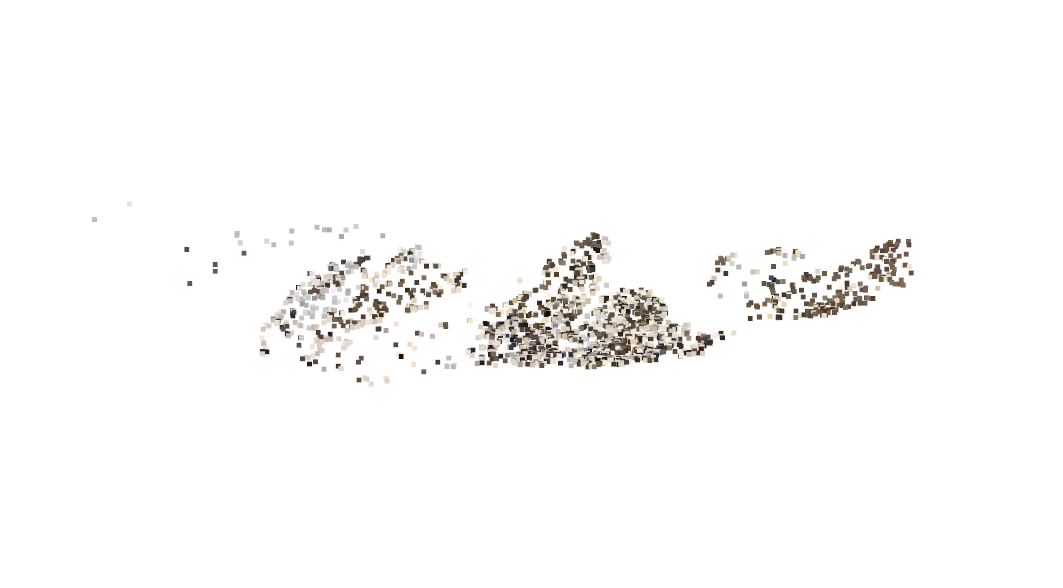
\includegraphics[width=\columnwidth]{3d reconstruction images/SIFT pairwise point cloud.png}
    \caption{Sparse 3D reconstruction obtained from the Palm Desert image pair.
    The reconstructed points capture recognizable scene structure, including
    the main hillside, while remaining distributed throughout the surrounding
    scene.}
    \label{fig:palm_desert_sparse_reconstruction}
\end{figure}

As shown in Figure~\ref{fig:palm_desert_sparse_reconstruction}, the resulting point cloud is sparse and does not form a continuous surface. Nevertheless, recognizable scene structure, including the main hillside visible in the input images, can be identified in the reconstruction. Additional reconstructed points are distributed across the surrounding scene, reflecting the feature-based nature of the approach rather than a dense surface reconstruction.


\subsubsection{Experimental Dense Reconstruction}

In addition to the sparse SIFT-based reconstruction, an experimental dense
stereo module was investigated. This module is intentionally treated as an
optional component rather than as a required stage of the main
feature-based reconstruction pipeline.

The \code{DenseReconstructor} operates on a single image pair and reuses the
relative rotation and translation already estimated during the feature-based
pipeline. The images are first downscaled to reduce computational cost and
their intrinsic matrix is scaled accordingly.
The pair is then rectified using OpenCV's
\code{cv2.stereoRectify()}, after which dense disparity is estimated using
\code{StereoSGBM}. The resulting disparity map is converted into 3D
coordinates using \code{cv2.reprojectImageTo3D()} and the reprojection matrix
obtained during rectification.
The module additionally performs validity checks and robust depth filtering
based on the Median Absolute Deviation (MAD). RGB values are sampled from the
rectified reference image and associated with the resulting 3D points.
This approach can produce substantially denser geometry than the sparse
feature-based reconstruction because depth is estimated over a large number
of image pixels rather than only at selected SIFT correspondences.

However, experiments showed that the dense reconstruction was not equally
reliable for all image pairs. Its quality depended strongly on the relative
camera motion, image overlap, scene texture, disparity distribution, and
quality of the estimated relative pose. Some pairs produced meaningful dense
geometry, whereas other pairs generated distorted or geometrically incorrect
structures.
For this reason, the dense stereo implementation remains experimental. It
was not considered necessary for the subsequent processing stages because
the sparse feature-based reconstruction already provides a set of 3D points
suitable for operations such as point cloud registration. The dense module
can therefore be evaluated or improved independently without becoming a
dependency of the main reconstruction workflow.

\subsection{OpenMVG/OpenMVS Reconstruction Pipeline}
\label{sec:openmvg_openmvs_pipeline}

To evaluate an established Structure-from-Motion (SfM) and multi-view stereo (MVS) reconstruction backend, a second reconstruction implementation was developed in \code{src_v2/}. Unlike the custom OpenCV-based reconstruction pipeline described previously, this implementation does not reproduce the individual SfM algorithms directly. Instead, Python provides the configuration, process orchestration, file management, and visualization interface, while the computational reconstruction stages are delegated to OpenMVG and OpenMVS. This pipeline is intentionally maintained as a separate reconstruction alternative. In particular, it is not an additional registration stage of the main DentaVision reconstruction pipeline: OpenMVG performs its own camera registration and SfM reconstruction as part of the established pipeline.

\subsubsection{Motivation for Using an Established SfM Pipeline}

The original reconstruction implementation was developed using OpenCV in order to expose and control the individual components of the SfM process, including SIFT feature extraction, feature matching, geometric verification, relative pose estimation, track construction, triangulation, landmark management, and bundle adjustment. This approach is useful for understanding the reconstruction process and for experimenting with individual algorithms, but it also requires substantial implementation and maintenance effort. In contrast, OpenMVG provides an established implementation of the complete sparse SfM workflow, including feature processing, matching, geometric filtering, camera estimation, triangulation, and optimization. The purpose of introducing OpenMVG was therefore not to replace the custom implementation, but to provide an alternative reconstruction backend in which the project could evaluate a more complete and established SfM implementation without having to reimplement the underlying reconstruction algorithms.

This distinction is also relevant when interpreting later experiments. Although OpenMVG provides the complete SfM framework, the feature extraction stage used by the project remains SIFT. Consequently, the use of an established SfM implementation does not eliminate limitations originating from the input features. In particular, scenes or images containing insufficient distinctive features can still present difficulties for feature matching and subsequent reconstruction. This makes the OpenMVG pipeline useful not only as a reconstruction backend, but also as an independent reference for evaluating the limitations of feature-based reconstruction.

\subsubsection{OpenMVG Pipeline}

The OpenMVG integration is implemented as a thin Python wrapper around the OpenMVG command-line applications. The project configuration is centralized in \code{src_v2/config/settings.py}, where the input image directory, OpenMVG installation, sensor-width database, output directories, feature extraction parameters, matching parameters, camera configuration, and SfM configuration are defined. Machine-dependent paths, including the input image directory and external software installations, are loaded from the project's \code{.env} file, while the OpenMVG executable directory and sensor-width database are derived from \code{OPENMVG_ROOT}. This keeps the reconstruction code independent of a particular installation path and allows camera- and dataset-dependent parameters to be changed without modifying the reconstruction pipeline itself.

\begin{figure}[H]
\centering
\begin{tikzpicture}[
node distance=0.5cm,
process/.style={
rectangle,
rounded corners,
draw,
align=center,
minimum width=5.2cm,
minimum height=0.8cm
},
arrow/.style={
-{Latex[length=2mm]},
thick
}
]

    \node[process] (input) {Input Images};
    \node[process, below=of input] (listing) {SfM Image Listing};
    \node[process, below=of listing] (features) {SIFT Feature Extraction};
    \node[process, below=of features] (matching) {Feature Matching};
    \node[process, below=of matching] (filtering) {Geometric Filtering};
    \node[process, below=of filtering] (sfm) {Incremental SfM};
    \node[process, below=of sfm] (sparse) {Sparse Reconstruction};
    \node[process, below=of sparse] (color) {Point Color Computation};
    \node[process, below=of color] (colored) {Colored Sparse Point Cloud};
    \node[process, below=of colored] (conversion) {OpenMVG/OpenMVS Conversion};
    \node[process, below=of conversion] (dense) {OpenMVS Dense Reconstruction};
    \node[process, below=of dense] (output) {Dense Point Cloud};

    \draw[arrow] (input) -- (listing);
    \draw[arrow] (listing) -- (features);
    \draw[arrow] (features) -- (matching);
    \draw[arrow] (matching) -- (filtering);
    \draw[arrow] (filtering) -- (sfm);
    \draw[arrow] (sfm) -- (sparse);
    \draw[arrow] (sparse) -- (color);
    \draw[arrow] (color) -- (colored);
    \draw[arrow] (colored) -- (conversion);
    \draw[arrow] (conversion) -- (dense);
    \draw[arrow] (dense) -- (output);

\end{tikzpicture}
\caption{End-to-end OpenMVG/OpenMVS reconstruction workflow.}
\label{fig:openmvg-openmvs-workflow}

\end{figure}

The sparse stage is coordinated by
\code{ReconstructionPipeline.run_sparse()}. First,
\code{openMVG_main_SfMInit_ImageListing} creates the initial
\code{sfm_data.json} from the input images and the configured camera
parameters. Camera-dependent values are centralized in
\code{settings.py}. When explicit intrinsic parameters are available, the
configured focal length and principal point are passed directly to OpenMVG.
If explicit focal-length information is not provided, OpenMVG can instead
use its sensor-width database together with the available image metadata to
initialize the camera intrinsics. This allows the same reconstruction
pipeline to be used with different cameras and image sets without requiring
changes to the reconstruction logic.


Feature extraction is then performed by
\code{openMVG_main_ComputeFeatures}. The project uses SIFT with the
\code{NORMAL} descriptor preset and configures 16 processing threads. The
resulting feature regions and descriptors are subsequently used by
\code{openMVG_main_ComputeMatches}, with a matching ratio configured in
\code{settings.py}. The resulting \code{matches.putative.bin} file contains
the initial feature correspondences.

These matches are subsequently passed to
\code{openMVG_main_GeometricFilter}, which uses the geometric model
configured by the project to remove correspondences that are inconsistent
with the estimated camera geometry. The selected geometric model is therefore
also treated as a configuration parameter rather than being hard-coded into
the reconstruction pipeline. The filtered correspondences are stored as
\code{matches.f.bin}.

The verified matches are then provided to
\code{openMVG_main_SfM}. The configured SfM engine is
\code{INCREMENTAL}, so OpenMVG progressively reconstructs the camera poses
and sparse 3D structure from the available image correspondences. The
reconstruction produces the OpenMVG SfM representation under
\code{output/openmvg/sfm/}, including \code{sfm_data.bin}. Finally,
\code{openMVG_main_ComputeSfM_DataColor} is used to generate the colored
sparse point cloud \code{cloud_and_poses.ply}. The visualization layer can
consume this point cloud without being coupled to the internal OpenMVG
representation.

The Python implementation deliberately keeps process execution separate from
reconstruction logic. The generic \code{run_command()} helper validates
executable paths, constructs and prints the generated command, and invokes
the external process using \code{subprocess.run(..., check=True)}.
Consequently, OpenMVG failures are propagated to the Python pipeline instead
of allowing subsequent stages to operate on invalid intermediate data. The
same abstraction is reused for the OpenMVS stage.

\subsubsection{Dense Reconstruction with OpenMVS}

OpenMVG provides the sparse reconstruction, whereas dense reconstruction is
delegated to OpenMVS. The implementation separates this process into two
independent operations: \code{prepare_dense()} converts the existing OpenMVG
reconstruction into an OpenMVS scene, while \code{run_dense()} performs the
actual dense reconstruction. This separation allows an existing scene to be
reused without repeating the sparse reconstruction or the scene conversion.

The scene preparation stage uses
\code{openMVG_main_openMVG2openMVS.exe}. Its primary input is the OpenMVG
reconstruction \code{sfm_data.bin}, and it generates
\code{output/openmvs/scene.mvs} together with the associated undistorted image
data. The resulting scene acts as the interface between the sparse OpenMVG
representation and the OpenMVS dense reconstruction stage. The implementation
also ensures that the image references required by the scene remain
accessible when OpenMVS loads the scene; the working directory used for the
dense reconstruction is therefore set to the directory containing the scene.

Dense reconstruction is performed by \code{DensifyPointCloud.exe}. The
generated point cloud is stored as
\code{output/openmvs/dense/pointcloud.ply}. The implementation supports CUDA
processing while retaining a CPU fallback. With the current configuration,
\code{OPENMVS_CUDA_DEVICE=None}, OpenMVS is first invoked with automatic GPU
selection (\code{-1}); if that attempt fails, the operation is retried using
CPU processing (\code{-2}). A specific CUDA device can alternatively be
configured, in which case the selected device is attempted first, followed by
automatic GPU selection and CPU processing. If a failed processing attempt
leaves an output file behind, that file is removed before the next attempt so
that an incomplete reconstruction cannot be mistaken for a successful
result.

The resulting architecture therefore separates the responsibilities of the
two reconstruction backends: OpenMVG performs feature-based sparse SfM and
produces camera poses and sparse 3D structure, while OpenMVS uses that
calibrated scene to generate a substantially denser point cloud. Camera
configuration and other dataset-dependent parameters remain external to the
reconstruction logic, allowing the same pipeline implementation to be reused
with different input image sets by modifying the project settings. Python
remains responsible for coordinating these stages and managing their
intermediate files rather than implementing the underlying SfM or MVS
algorithms.

\subsubsection{3D Reconstruction Results on the Palm Desert Dataset}
\label{sec:palm_desert_reconstruction_results}

The sparse reconstruction generated by OpenMVG was subsequently used as
input for dense reconstruction with OpenMVS. The input scene contained
21 calibrated images and 83,416 sparse 3D points. OpenMVS estimated
depth maps for all 21 views, enforced geometric consistency between
the views, and fused the resulting depth maps into a dense point cloud.
After depth-map fusion, filtering, and trimming to the estimated region
of interest, the final dense point cloud contained 1,753,190 3D points.
This corresponds to approximately 21 times the number of points in the
original sparse reconstruction, providing a substantially denser
representation of the reconstructed scene.

\begin{table}[H]
    \centering
    \caption{OpenMVG/MVS dense reconstruction results.}
    \label{tab:openmvs_dense_results}
    \begin{tabular}{lr}
        \hline
        \textbf{Metric} & \textbf{Result} \\
        \hline
        Calibrated images & 21 \\
        Sparse points & 83,416 \\
        Dense points & 1,753,190 \\
        Dense/Sparse ratio & $\approx 21\times$ \\
        \hline
    \end{tabular}
\end{table}

Figure~\ref{fig:sparse_dense_comparison} provides a visual comparison
between the sparse reconstruction produced by OpenMVG and the final
dense point cloud generated by OpenMVS. In the sparse reconstruction,
the green markers represent the estimated camera positions, whose
distribution reflects the relative camera motion recovered from the
image correspondences. The coherent camera trajectory provides a
visual indication that the feature tracks and pose estimation successfully
captured the camera movement throughout the sequence. The comparison
also illustrates the substantial increase in point density obtained
during the dense reconstruction stage while preserving the overall
geometry of the reconstructed scene.

\begin{figure}[H]
    \centering
    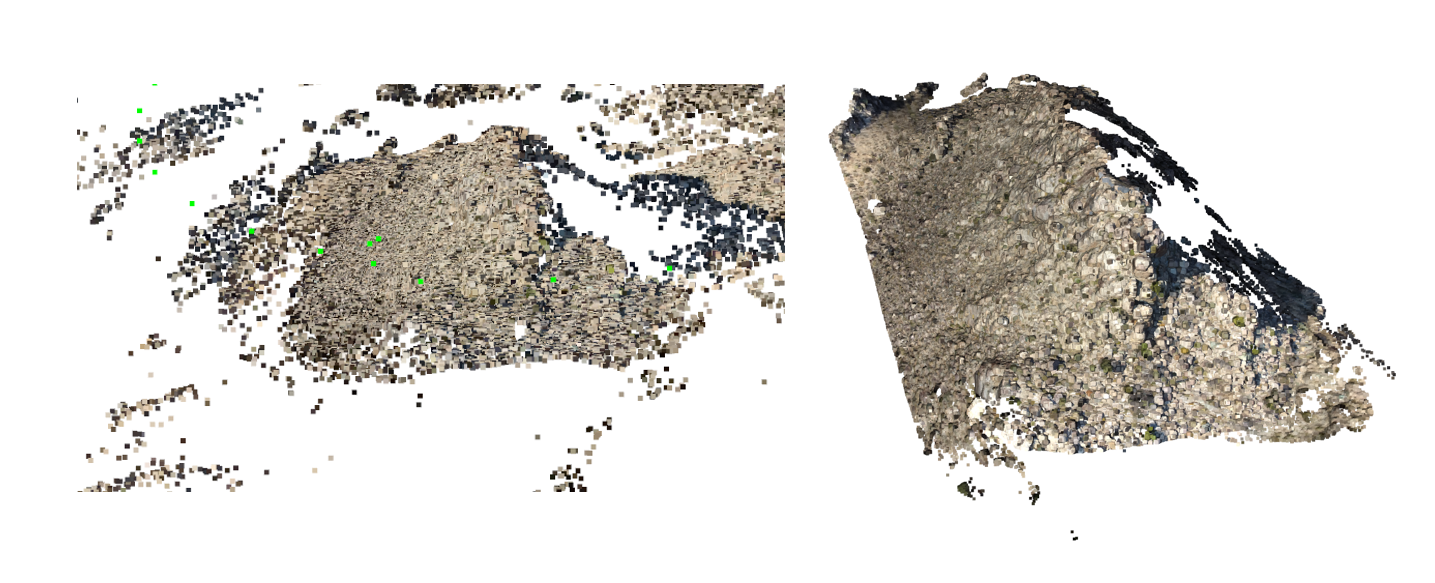
\includegraphics[width=\columnwidth]{3d reconstruction images/OpenMVG-MVS point clouds.png}
    \caption{Comparison between the sparse reconstruction generated by
    OpenMVG (left) and the dense point cloud generated by OpenMVS
    (right).}
    \label{fig:sparse_dense_comparison}
\end{figure}


\subsection{Evaluation on Low-Texture Scenes}

The feature-based reconstruction pipeline was initially developed and evaluated
using the Palm Desert Micro dataset provided through the OpenMVG image dataset
repository~\cite{openmvgImageDatasets}. While this dataset was suitable for
developing the reconstruction workflow, it did not sufficiently represent the
challenging visual conditions that may be encountered during dental
reconstruction, particularly in regions with limited distinctive visual
features. Therefore, an additional evaluation was required to investigate how
the current reconstruction approach behaves when the available image texture
is insufficient to establish a large number of reliable correspondences.

To investigate this limitation, additional experiments were performed using
the Middlebury Stereo 2006 datasets~\cite{scharstein2007learning,hirschmuller2007evaluation}.
The evaluation focused on four scenes with different visual characteristics:
\textit{Midd1}, \textit{Midd2}, \textit{Monopoly}, and \textit{Plastic}.
The four scenes were evaluated first using the implemented SIFT-based pairwise
pipeline and subsequently using OpenMVG for Structure-from-Motion. This
provided both a direct evaluation of the implemented feature-based approach
and an additional reference using an independent SfM implementation.

\subsubsection{Motivation for the Middlebury Dataset}

The Middlebury Stereo 2006 dataset was selected because it provides
well-established stereo scenes with controlled imaging conditions and
available ground-truth disparity data~\cite{scharstein2007learning,hirschmuller2007evaluation}.
The images are rectified, and the dataset provides stereo information for
specific image views, including \code{view1.png} and \code{view5.png}.
For the pairwise evaluation, these two views were used as an independent image
pair for each scene. Although the Middlebury scenes originate from a
multi-view stereo benchmark, the implemented pairwise experiment only receives
the selected two images. Consequently, the reconstruction performed by the
DentaVision pipeline remains a two-view reconstruction and does not use the
additional views available in the dataset.
The four selected scenes expose the reconstruction process to different levels
of available local image structure. In particular, the \textit{Plastic} scene
contains substantially fewer distinctive features than the other evaluated
scenes and therefore provides a useful stress case for feature-based
reconstruction.

The purpose of this experiment was not to evaluate dense stereo reconstruction
at this stage. Instead, the initial objective was to establish a baseline for
the existing feature-based reconstruction approach and determine whether a
lack of detectable and matchable image features could become a limiting factor
for sparse 3D reconstruction.

\subsubsection{SIFT Reconstruction on Middlebury Images}

The existing pairwise reconstruction pipeline was applied to
\code{view1.png} and \code{view5.png} for each of the four scenes without
changing its feature-based reconstruction architecture. For each image pair,
the number of detected SIFT keypoints, the number of matches remaining after
the Lowe ratio test, the number of RANSAC inliers, the resulting inlier ratio,
and the number of reconstructed 3D points were recorded.

The inlier ratio was computed as

\begin{equation}
\text{Inlier Ratio} =
\frac{\text{RANSAC Inliers}}
{\text{Good Matches}}
\times 100.
\end{equation}

An important change compared with the initial Middlebury experiment concerns
the camera calibration. The original project configuration had been defined
for the Palm Desert Micro dataset. The Middlebury experiments were therefore
rerun using the appropriate Middlebury camera parameters rather than the
Palm Desert calibration. This prevents the camera model from introducing an
additional source of error into the relative pose and triangulation stages.

The resulting measurements are summarized in
Table~\ref{tab:middlebury_sift_results}.

\begin{table}[H]
\centering
\caption{Results of the SIFT-based pairwise reconstruction on the Middlebury scenes.}
\label{tab:middlebury_sift_results}
\resizebox{\columnwidth}{!}{%
\begin{tabular}{lrrrrrr}
\toprule
Dataset & View 1 KP & View 5 KP & Good Matches &
Inliers & Inlier Ratio & 3D Points \\
\midrule
Midd1    & 621 & 610 & 344 & 311 & 90.41\% & 311 \\
Midd2    & 575 & 572 & 333 & 306 & 91.89\% & 306 \\
Monopoly & 684 & 701 & 414 & 287 & 69.32\% & 287 \\
Plastic  & 127 & 67  & 43  & 9   & 20.93\% & 9   \\
\bottomrule
\end{tabular}%
}
\end{table}

The first three scenes produced several hundred usable correspondences.
\textit{Midd1} produced 311 RANSAC inliers from 344 good descriptor matches,
corresponding to an inlier ratio of 90.41\%. Similarly, \textit{Midd2} produced
306 inliers from 333 good matches, resulting in an inlier ratio of 91.89\%.
The corresponding triangulation stages produced 311 and 306 reconstructed
points, respectively.
\textit{Monopoly} produced the largest number of candidate descriptor
matches, with 414 good matches. However, only 287 survived geometric
verification, resulting in a lower inlier ratio of 69.32\%. Nevertheless, the
resulting reconstruction still contained 287 3D points.
In contrast, \textit{Plastic} showed a substantial reduction in feature
availability. Only 127 keypoints were detected in \code{view1.png} and 67 in
\code{view5.png}. This resulted in only 43 good descriptor matches, of which
9 remained after RANSAC. The resulting inlier ratio was therefore only
20.93\%, and the triangulation stage produced only 9 3D points.

These results indicate that the degradation observed for \textit{Plastic}
occurs progressively throughout the feature-based reconstruction process. The
scene first provides substantially fewer detectable local features, which
limits the number of candidate descriptors and correspondences. The reduced
number of correspondences is then accompanied by lower geometric consistency,
ultimately leaving too few points for a substantial sparse reconstruction.

\subsubsection{OpenMVG and OpenMVS Evaluation}

To determine whether the observed limitations were specific to the implemented
pairwise reconstruction pipeline, the same four Middlebury scenes were also
processed using OpenMVG for Structure-from-Motion reconstruction. Unlike the
implemented pairwise pipeline, OpenMVG performs multi-view Structure-from-Motion
and therefore requires multiple images to estimate the camera motion and
reconstruct the scene. Consequently, all seven available views of each Middlebury
scene were used for the OpenMVG evaluation.
Therefore, the comparison is not intended to determine which implementation performs better, but rather to assess whether a multi-view SfM approach can provide sufficient sparse structure under the same challenging scene conditions. The SIFT-based experiment uses
only \code{view1.png} and \code{view5.png}, whereas OpenMVG uses the complete
seven-view sequence available for each scene. The two experiments are
therefore evaluated separately, with the OpenMVG results serving as an
additional assessment of the sparse reconstruction and its suitability as
input for subsequent dense reconstruction.
In particular, the number of OpenMVG tracks should not be interpreted as
directly comparable to the number of pairwise SIFT inliers. Instead, the
OpenMVG results were used to determine whether a sparse reconstruction could
be established and whether sufficient sparse structure was available for
subsequent dense reconstruction.

OpenMVG successfully produced a sparse reconstruction for all four evaluated
scenes. However, the amount of reconstructed structure varied considerably
between datasets. The recorded results are summarized in
Table~\ref{tab:middlebury_openmvg_results}.


\begin{table}[H]
\centering
\caption{OpenMVG sparse reconstruction results on the Middlebury scenes.}
\label{tab:middlebury_openmvg_results}
\resizebox{\columnwidth}{!}{%
\begin{tabular}{lrr}
\toprule
Dataset & Reconstructed Tracks / 3D Points & Calibrated Cameras \\
\midrule
Midd1    & 129 & 7 / 7 \\
Midd2    & 32  & 7 / 7 \\
Monopoly & 4   & 7 / 7 \\
Plastic  & 29  & 3 / 7 \\
\bottomrule
\end{tabular}%
}
\end{table}

The OpenMVG results demonstrate that successful camera calibration and sparse
reconstruction do not necessarily imply that a sufficiently dense set of
points is available for subsequent processing. For example, \textit{Midd1}
resulted in 129 reconstructed tracks with all seven input cameras calibrated,
whereas \textit{Monopoly} resulted in only four reconstructed tracks despite
all seven cameras being calibrated.
For \textit{Plastic}, OpenMVG reconstructed 29 tracks and calibrated three of
the seven input cameras. The corresponding residual statistics showed a mean
reprojection residual of approximately 0.18 pixels and a median of
approximately 0.10 pixels. These low residual values indicate that the
surviving tracks were geometrically consistent, but they do not imply
sufficient scene coverage.
The sparse reconstructions were subsequently passed to OpenMVS for dense
reconstruction. OpenMVS was not able to successfully complete the dense
reconstruction for the evaluated scenes. The observed behavior was
investigated through repeated tests to distinguish a possible implementation
problem from a limitation of the input reconstruction.
The experiments consistently showed that OpenMVG was able to produce a sparse
point cloud before the OpenMVS stage. Therefore, the observed OpenMVS failure
was not attributed to the absence of an OpenMVG reconstruction. Instead, the
results are consistent with the hypothesis that the sparse reconstructions
contained too few reliable points and tracks to provide sufficient geometric
support for successful densification.

This interpretation should be considered an experimental observation rather
than a formally isolated causal result. The experiments did not independently
vary the number of sparse points while keeping all other conditions constant.
Nevertheless, the combination of sparse OpenMVG reconstructions and the
subsequent failure of dense reconstruction provides evidence that insufficient
sparse scene structure is a plausible limitation of the SfM-to-MVS approach
for these scenes.

\subsubsection{Implications for Dental Reconstruction}

The Middlebury experiments demonstrate an important limitation of
feature-based sparse reconstruction: its performance depends strongly on the
availability of distinctive and repeatable visual features.
These findings are relevant to dental reconstruction because dental surfaces
cannot be assumed to provide uniformly distinctive local image features.
Regions with limited local texture may result in fewer reliable feature
correspondences, while specular reflections and other appearance variations
can further complicate feature matching. A reconstruction approach that relies
exclusively on sparse feature correspondences may therefore provide
insufficient spatial coverage in some regions of the scene.

The experiments do not establish that SIFT or feature-based reconstruction is
generally unsuitable for dental images. Instead, they identify a specific
limitation of the current approach: reconstruction quality and coverage can
degrade substantially when the available visual features are insufficient.
Consequently, the Middlebury evaluation established the SIFT-based sparse
reconstruction as a baseline and motivated the investigation of dense stereo
correspondence as a complementary reconstruction strategy. The subsequent
evaluation of StereoSGBM is therefore presented separately, with the
\textit{Plastic} scene providing a particularly useful test case for dense
stereo because ground-truth disparity is available.

\subsection{Stereo Reconstruction with SGBM}

As an alternative to the feature-based reconstruction pipeline, DentaVision includes a dense stereo reconstruction approach based on OpenCV's Stereo Semi-Global Block Matching (StereoSGBM). This approach was evaluated using the Middlebury 2006 Plastic stereo dataset, which provides a calibrated and already rectified stereo pair together with a ground-truth disparity map. The stereo implementation is organized into separate components for disparity estimation, disparity validation, depth computation, and 3D point cloud reconstruction.

\subsubsection{StereoSGBM Implementation}

The disparity estimation stage is implemented by the \code{StereoMatcher} class in \longcode{src/pipeline/stereo/matcher.py}. It encapsulates OpenCV's \code{cv2.StereoSGBM_create()} and computes a dense disparity map from a pair of rectified stereo images. The implementation accepts either grayscale or BGR images. BGR images are converted to grayscale before matching, while grayscale images are used directly. The two input images are required to have identical spatial dimensions.

The matcher exposes the main StereoSGBM parameters through its constructor. The default configuration uses a minimum disparity of 0 and searches 128 disparity levels. The matching block size is set to 5 pixels, with a uniqueness ratio of 10, a speckle window size of 100 pixels, a speckle range of 2, and a maximum left-right disparity difference of 1 pixel. The implementation uses the \code{STEREO_SGBM_MODE_SGBM_3WAY} mode. The smoothness penalties are derived from the block size as \(P_1=8b^2\) and \(P_2=32b^2\), where \(b\) denotes the selected block size. Input validation also ensures that the number of disparity levels is a positive multiple of 16 and that the block size is a positive odd number.

OpenCV internally stores StereoSGBM disparity values with a fixed scale factor of 16. Therefore, the implementation converts the output to floating-point pixel units by dividing the computed disparity map by 16. The resulting array has the same spatial resolution as the input images and is represented using \code{float32}.

For the Middlebury evaluation, the images used were the ThirdSize versions of \code{view1.png} and \code{view5.png}, with a resolution of \(423\times370\) pixels. The dataset images are already rectified and have radial distortion removed, so no additional stereo rectification or distortion correction is performed by the reconstruction pipeline. The corresponding camera configuration is therefore derived directly from the parameters provided by the dataset. The original focal length of 3740 pixels is scaled according to the ThirdSize image resolution, while the stereo baseline is 160 mm. The principal point is set to the center of the \(423\times370\) image. A corresponding \(4\times4\) reprojection matrix \(Q\) is also defined for the Middlebury stereo geometry and supplied to the 3D reconstruction component.

\subsubsection{Disparity Validation and Depth Reconstruction}

After disparity estimation, the resulting map is passed to the \code{StereoValidator}. This component is intentionally separated from the reconstruction stages and currently performs two basic validity checks: disparity values must be finite and strictly greater than zero. The result is a boolean validity mask with the same dimensions as the disparity map. This separation allows additional validation strategies, such as left-right consistency checks, to be introduced later without changing the depth or point cloud reconstruction components.

The validated disparity can subsequently be used to estimate depth. This functionality is implemented by the \code{DepthReconstructor}, which applies the stereo depth relationship \(Z=fB/d\) to all finite, positive disparity values. Invalid values are assigned a depth of zero. The focal length and baseline are provided to the component externally, and the resulting depth map uses the same physical unit as the supplied baseline.

For the Middlebury dataset, an additional disparity offset has to be considered during reconstruction. The ThirdSize images are cropped versions of the original images, and the dataset specifies a minimum disparity value of \(d_{\min}=280\) pixels. Consequently, the disparity estimated by StereoSGBM is offset before it is used for the Middlebury reconstruction:

\begin{equation}
d_{\mathrm{reconstruction}}
=
d_{\mathrm{SGBM}}
+
d_{\min}.
\label{eq:disparity_reconstruction}
\end{equation}

With the baseline expressed in millimeters, the resulting depth values are correspondingly expressed in millimeters.

The final 3D reconstruction is handled by the \code{StereoReconstructor}. Rather than explicitly computing the three-dimensional coordinates from individual image coordinates and depth values, this component uses OpenCV's \code{cv2.reprojectImageTo3D()} function. The function receives the reconstruction disparity and an externally supplied \(4\times4\) reprojection matrix \(Q\). Keeping \(Q\) outside the reconstruction class makes the component independent of a specific camera or dataset.

The complete disparity map is first reprojected into 3D space. The validation mask is then used to select only the pixels considered valid for reconstruction. Any resulting 3D coordinates that are not finite are discarded. The corresponding colors are obtained from the left stereo image, converted from BGR to RGB, and normalized to the range \([0,1]\). The resulting points and colors are stored in the common \code{PointCloud} representation used by the rest of the reconstruction pipeline.

The resulting processing flow can therefore be summarized as:

\begin{figure}[H]
    \centering
    \begin{tikzpicture}[
        node distance=0.5cm,
        block/.style={
            draw,
            rounded corners,
            align=center,
            minimum height=0.5cm,
            minimum width=2.5cm
        },
        arrow/.style={
            -{Stealth},
            thick
        }
    ]

        \node[block] (input) {Left/Right Images};
        \node[block, below=of input] (sgbm) {StereoSGBM};
        \node[block, below=of sgbm] (disparity) {Disparity};
        \node[block, below=of disparity] (validator) {StereoValidator};
        \node[block, below=of validator] (mask) {Valid Mask};
        \node[block, below=of mask] (depth) {Depth / 3D Reprojection};
        \node[block, below=of depth] (pointcloud) {PointCloud};

        \draw[arrow] (input) -- (sgbm);
        \draw[arrow] (sgbm) -- (disparity);
        \draw[arrow] (disparity) -- (validator);
        \draw[arrow] (validator) -- (mask);
        \draw[arrow] (mask) -- (depth);
        \draw[arrow] (depth) -- (pointcloud);

    \end{tikzpicture}
    \caption{Dense stereo reconstruction pipeline using StereoSGBM.}
    \label{fig:sgbm_pipeline}
\end{figure}

\subsubsection{Quantitative and Qualitative Results}

The StereoSGBM implementation was evaluated quantitatively against the ground-truth disparity provided by the Middlebury Plastic dataset. Three matching block sizes, 3, 5, and 7 pixels, were tested while keeping the remaining StereoSGBM parameters unchanged. The results are summarized in Table~\ref{tab:stereosgbm_block_sizes}.

\begin{table}[H]
\centering
\caption{StereoSGBM disparity accuracy for different block sizes on the Middlebury Plastic dataset.}
\label{tab:stereosgbm_block_sizes}
\resizebox{\columnwidth}{!}{%
\begin{tabular}{c|ccccc}
\hline
Block size & MAE (px) & Median AE (px) & $>1$ px & $>2$ px & $>5$ px \\
\hline
3 & 2.81 & 0.60 & 37.78\% & 27.27\% & 18.64\% \\
5 & 2.91 & 0.60 & 39.06\% & 29.23\% & 20.13\% \\
7 & \textbf{2.66} & 0.60 & 38.30\% & 28.27\% & \textbf{18.91\%} \\
\hline
\end{tabular}%
}
\end{table}

Among the tested configurations, a block size of 7 produced the lowest mean absolute error of 2.66 pixels and was therefore selected for the subsequent reconstruction. Although the improvement over the other configurations was small, it provided the best quantitative result, while the median absolute error remained unchanged at 0.60 pixels. Nevertheless, the disparity estimates still contained a considerable number of local errors: \(38.30\%\) of the valid comparison pixels had an absolute error greater than 1 pixel, and \(18.91\%\) exceeded 5 pixels.

For the subsequent reconstruction, the selected configuration produced a disparity map of \(370\times423\) pixels. The \code{StereoValidator} classified \(45.94\%\) of the image pixels as valid, excluding disparities that were non-finite or not strictly positive. This value reflects the validity criterion of the implementation rather than the accuracy of the disparity estimates.
After applying the Middlebury \(d_{\min}\) offset, the reconstructed disparity values corresponded to depths between approximately 1.73 m and 2.13 m, with a mean depth of 1.84 m. The reprojection produced 71,904 valid 3D points, with no additional point loss caused by non-finite coordinates. Thus, the resulting point cloud contained one 3D point for each valid disparity pixel in this evaluation.


\begin{figure}[H]
\centering
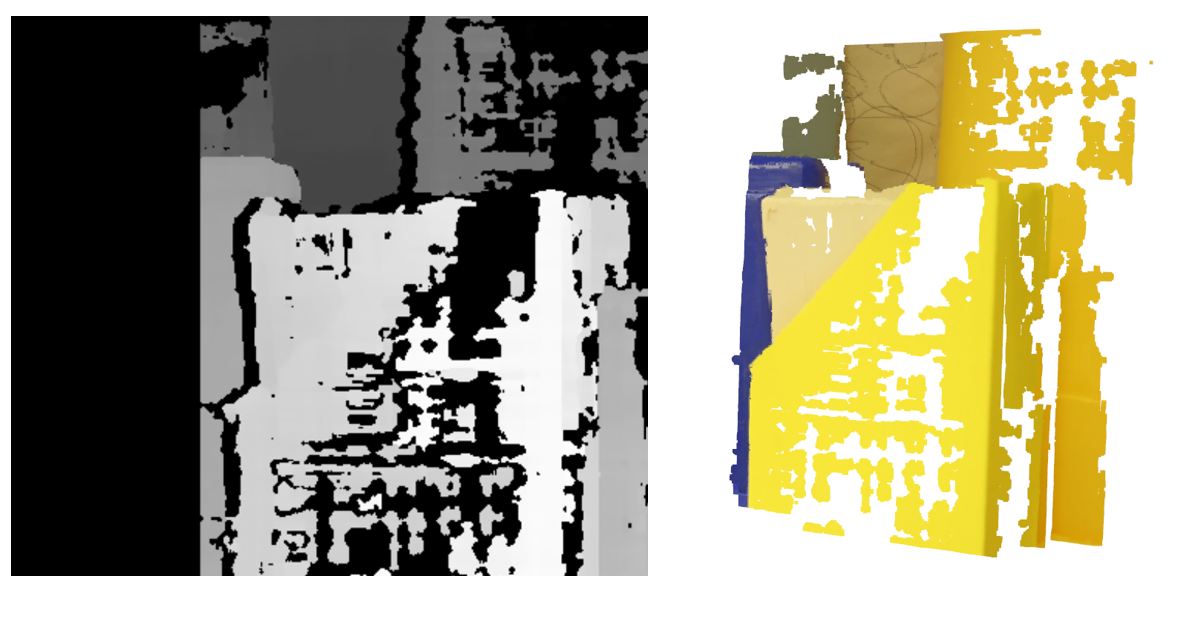
\includegraphics[width=0.8\linewidth]{3d reconstruction images/SGBM output.png}
\caption{Dense stereo reconstruction of the Middlebury Plastic
ThirdSize image pair using StereoSGBM. The left image shows the
estimated disparity map, while the right image shows the corresponding
colored 3D point cloud reconstructed from the disparity.}
\label{fig:sgbm_disparity_pointcloud}
\end{figure}


As shown in Figure~\ref{fig:sgbm_disparity_pointcloud}, the estimated
disparity provides a dense representation of the scene's depth structure.
The main regions of the scene are recovered consistently, while some
areas contain invalid or missing disparity values. These regions indicate
locations where a reliable disparity estimate was not obtained. The
corresponding colored point cloud provides a three-dimensional
representation of the reconstructed scene while retaining the color
information. The recovered spatial structure is consistent with the
disparity estimation, although the density and completeness of the point
cloud depend directly on the reliability and spatial coverage of the
underlying disparity map.


\subsection{IGEV Stereo Reconstruction with OpenStereo}

\subsubsection{Overview}

The project integrates the IGEV stereo matching model through the external
OpenStereo framework to provide dense stereo disparity for 3D reconstruction.
Unlike the custom StereoSGBM implementation, IGEV is a pretrained
deep-learning stereo model. OpenStereo provides the IGEV implementation,
configuration, preprocessing, and inference functionality, while DentaVision
integrates its disparity output into the existing stereo reconstruction
pipeline.

\subsubsection{Motivation for Using OpenStereo}

The project uses IGEV through the OpenStereo framework rather than integrating
the original IGEV implementation directly.
The main reason for this choice is to keep the stereo matching component
flexible. OpenStereo provides a common framework for multiple stereo matching
models, allowing the project to use IGEV while keeping the integration
independent from a single model implementation.
This makes it possible to evaluate or replace the stereo matching method in
the future with other models supported by OpenStereo without requiring major
changes to the downstream reconstruction pipeline. The
\code{IGEVMatcher} isolates the framework-specific details, while the rest of
the pipeline only receives a dense disparity map.
Therefore, OpenStereo is used not only as the implementation source for IGEV,
but also as an abstraction layer that keeps the project open to additional
deep-learning stereo models in the future.

\subsubsection{Preprocessing and Padding}

The evaluation transform configured by OpenStereo can pad the input images to
dimensions compatible with the IGEV network. The matcher stores the original
image dimensions before preprocessing and removes the added padding after
inference.
For the configured transform, padding is added to the top and right sides.
Consequently, the original image corresponds to the upper-left region of the
model output. The matcher removes the padded rows from the top and the padded
columns from the right before returning the disparity.
The final disparity therefore has exactly the same dimensions as the original
input image. This is required so that the disparity remains spatially aligned
with the left image during subsequent validation and 3D reconstruction.

\subsubsection{OpenStereo Integration}

OpenStereo is kept as an external dependency and is not included in the
DentaVision source tree. Both OpenStereo and IGEV checkpoint are configured through the \code{.env} file. They have separate variables, which keeps the OpenStereo installation and the pretrained checkpoint independent from each other.

The integration is implemented in
\code{src/pipeline/stereo/igev_matcher.py}. The \code{IGEVMatcher} acts as an
adapter between the DentaVision stereo pipeline and OpenStereo. During
initialization, it loads the OpenStereo configuration, assigns the configured
checkpoint, builds the IGEV model through OpenStereo, and creates the
evaluation transform defined by the selected configuration.
For each stereo pair, \code{compute()} validates the input images and their
dimensions, converts the OpenCV BGR images to RGB, and applies the OpenStereo
evaluation transform. The resulting tensors are batched and moved to the
selected device before IGEV inference is performed without gradient
computation. The predicted \code{disp_pred} is then extracted, converted to a
\code{float32} NumPy array, and any padding introduced by the OpenStereo
transform is removed before returning the disparity at the original image
resolution.


The matcher therefore exposes a simple interface to the rest of the project:

\begin{center}
\resizebox{\columnwidth}{!}{
\begin{tikzpicture}[
    node distance=1.2cm,
    box/.style={
        rectangle,
        draw,
        rounded corners,
        align=center,
        minimum width=3.8cm,
        minimum height= 1cm
    },
    arrow/.style={->, >=stealth}
]

\node[box] (input) {Left and right (rectified) images};
\node[box, right=1.8cm of input] (matcher)
{\code{IGEVMatcher.compute()}};
\node[box, right=1.8cm of matcher] (output)
{Dense disparity};

\draw[arrow] (input) -- (matcher);
\draw[arrow] (matcher) -- (output);

\end{tikzpicture}
}
\end{center}

The rest of the reconstruction pipeline therefore does not need to interact
directly with the OpenStereo trainer or the IGEV model implementation.


\subsubsection{Middlebury Evaluation}

The IGEV implementation was evaluated using the Plastic stereo pair from the
Middlebury dataset. The images have a resolution of $423 \times 370$ pixels.
The Middlebury ThirdSize ground-truth disparity is stored with a scale factor
of three. Therefore, the raw ground-truth values are divided by three before
comparison with the IGEV prediction.

The evaluation produced the following results:

\begin{table}[ht]
\centering
\caption{IGEV disparity accuracy on the Middlebury Plastic dataset.}
\label{tab:igev_disparity_accuracy}
\begin{tabular}{l r}
\hline
Metric & Result \\
\hline
Disparity minimum & 17.73 px \\
Disparity maximum & 64.95 px \\
Disparity mean & 45.10 px \\
Disparity median & 44.11 px \\
\hline
Valid comparison pixels & 156267 \\
Mean absolute error & 0.42 px \\
Median absolute error & 0.27 px \\
Maximum absolute error & 24.82 px \\
Mean signed error & -0.17 px \\
Median signed error & -0.12 px \\
Absolute error $> 1$ px & 7.64\% \\
Absolute error $> 2$ px & 1.05\% \\
Absolute error $> 5$ px & 0.20\% \\
\hline
\end{tabular}
\end{table}

The mean absolute error of $0.42$ pixels and median absolute error of
$0.27$ pixels show a close agreement between the IGEV prediction and the
Middlebury ground truth. Only $0.27\%$ of the compared pixels have an
absolute error greater than five pixels.

\subsubsection{Dense Reconstruction}

The predicted disparity was passed to the existing
\code{StereoValidator}, \code{DepthReconstructor}, and
\code{StereoReconstructor} components.
The current validation accepted all 156510 pixels,
resulting in a validity ratio of $100.00\%$.
The resulting depth values ranged from $3070.72$ mm to $11249.35$ mm, with a
mean of $5050.46$ mm and a median of $4522.90$ mm.
The final 3D reconstruction contained 156510 points. The point coordinates
have shape $(156510, 3)$ and the corresponding point colors have shape
$(156510, 3)$.

Figure~\ref{fig:igev_disparity_pointcloud} provides a visual representation
of the dense stereo result and the resulting 3D reconstruction. The
disparity captures the main depth structure of the scene, which is reflected
in the spatial organization of the reconstructed point cloud. Qualitatively,
the reconstruction appears largely complete, with few visible gaps or
inconsistencies relative to the scene represented in the input stereo pair.
The resulting point cloud therefore provides a coherent representation of
the observed scene structure.

\begin{figure}[H]
\centering
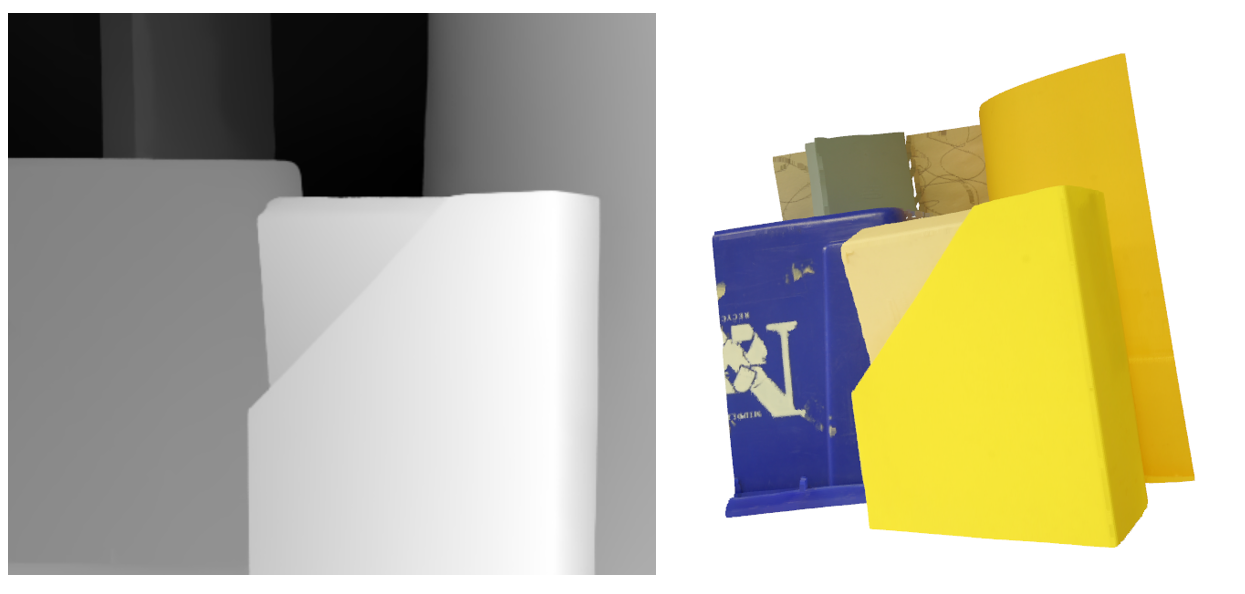
\includegraphics[width=0.8\linewidth]{3d reconstruction images/IGEV output.png}
\caption{Dense stereo result and 3D reconstruction obtained with IGEV
on the Middlebury Plastic stereo pair. The left image shows the
estimated disparity map, while the right image shows the corresponding
colored 3D point cloud reconstructed from the disparity.}
\label{fig:igev_disparity_pointcloud}
\end{figure}

The IGEV integration therefore provides a dense stereo backend that can be
used with the existing validation, depth reconstruction, and 3D
reconstruction components without requiring model-specific processing in
those stages.

\subsection{Comparative Evaluation}
\label{sec:comparative_evaluation}

The evaluated reconstruction approaches differ in their input requirements
and reconstruction principles. Consequently, a single quantitative metric
cannot be applied fairly to all four methods. The pairwise SIFT and
OpenMVG/OpenMVS approaches are instead considered primarily in terms of
their behavior and limitations observed during the low-texture evaluation,
while StereoSGBM and IGEV allow a direct quantitative comparison because
both estimate dense disparity from the same calibrated stereo pair.

\begin{table}[H]
    \centering
    \caption{Quantitative comparison of dense stereo reconstruction on the
    Middlebury Plastic dataset. For StereoSGBM, the results correspond to
    the best-performing block size of 7.}
    \label{tab:stereo_comparison}
    \begin{tabular}{lcc}
        \hline
        \textbf{Metric} & \textbf{StereoSGBM} & \textbf{IGEV} \\
        \hline
        Block size & 7 & -- \\
        Mean absolute error (px) & 2.66 & \textbf{0.42} \\
        Median absolute error (px) & 0.60 & \textbf{0.27} \\
        Error $>1$ px & 38.30\% & \textbf{7.64\%} \\
        Error $>2$ px & 28.27\% & \textbf{1.05\%} \\
        Error $>5$ px & 18.91\% & \textbf{0.20\%} \\
        \hline
    \end{tabular}
\end{table}

The quantitative evaluation shows a clear advantage of IGEV over
StereoSGBM on the Middlebury Plastic scene. IGEV achieved a mean absolute
disparity error of 0.42~px compared with 2.91~px for StereoSGBM, while the
median error decreased from 0.60~px to 0.27~px. The IGEV results also show
that only 0.27\% of the evaluated pixels have an absolute disparity error
greater than 5~px. Both methods produced disparity maps with comparable
overall disparity statistics, indicating that the difference is primarily
in the accuracy of the estimated disparity rather than in the recovered
disparity range.

More broadly, the experiments show that feature-based approaches can
provide useful sparse reconstructions when sufficient visual structure is
available, as demonstrated by the initial Palm Desert evaluation.
However, the Middlebury experiments exposed substantial limitations under
low-texture conditions. The use of OpenMVG's multi-view SfM formulation
does not fundamentally remove this limitation, since it still relies on
reliable image correspondences to establish the scene geometry. In
contrast, dense stereo methods directly estimate disparity from the
calibrated stereo pair and therefore do not require a sparse
feature-based scene representation. Between the two evaluated stereo
approaches, IGEV achieved substantially lower disparity error than
StereoSGBM on the Plastic scene and provided the most promising results
for the targeted stereo reconstruction scenario.

\subsection{Conclusion}

This work investigated several approaches for reconstructing three-dimensional geometry from image data within the DentaVision project. Feature-based reconstruction using SIFT provided a functional sparse reconstruction pipeline and demonstrated that reliable camera motion and 3D points can be obtained when sufficient visual structure is available. However, the experiments on the low-texture Middlebury Plastic dataset revealed clear limitations of feature-based methods in regions with little distinctive texture. The use of OpenMVG and OpenMVS confirmed that a multi-view SfM pipeline does not fully overcome this limitation when the input images do not provide sufficient visual correspondences.
Dense stereo methods proved more suitable for the low-texture scenario. StereoSGBM was able to produce a dense disparity map, but its accuracy remained limited, particularly in regions where local image structure was insufficient. In contrast, the IGEV-based stereo approach achieved substantially lower disparity errors on the same calibrated Middlebury stereo pair.
The Plastic stereo pair is particularly relevant to the intended DentaVision application because its predominantly low-texture surfaces provide a scenario that is more representative of the visual characteristics expected from dental surfaces than the highly textured Palm Desert dataset. Based on its strong quantitative performance in this evaluation, IGEV will be used as the basis for the stereo matching component of the DentaVision reconstruction pipeline. Its ability to produce accurate dense disparity in this challenging low-texture scenario makes it a particularly suitable approach for the intended application.